%%% Folie
\begin{frame}{Lernziele}
    \begin{itemize}
        \item Die verschiedenen Hardwarebausteine eines IoT-Systems kategorisieren
        \item Die physikalischen Grundlagen des elektrischen Stroms verstehen
        \item Die Begriffe \glqq{}Spannung\grqq{}, \glqq{}Stromstärke\grqq{} und
              \glqq{}Widerstand\grqq{} abgrenzen
        \item Schaltpläne lesen und nachvollziehen können
        \item Eigene mikrocontrollerbasierte Schaltungen entwickeln können
        \item Hierzu die Funktionsweise der wichtigsten Bausteine verstehen
        \item Sowie das Ohmsche Gesetz anwenden
        \item Die Hardwareschnittstellen des Raspberry Pi nutzen können
        \item Analoge und digitale Sensoren und Aktoren nutzen können
        \item Die Bedeutung und Funktionsweise serieller Kommunikation kennen
    \end{itemize}
\end{frame}

%-------------------------------------------------------------------------------
\section{Übersicht}
%-------------------------------------------------------------------------------

%%% Folie
{
    \setbeamertemplate{background canvas}{
        \includegraphics[height=\paperheight, width=\paperwidth]{2-hardwaredesign/img/bauteile}
    }

    \begin{frame}[plain]
    \end{frame}
}

%%% Folie
{
\small

\begin{frame}{Beispiel: Elementare Bauteile}
    \begin{columns}
        \column[b]{.25\textwidth}
        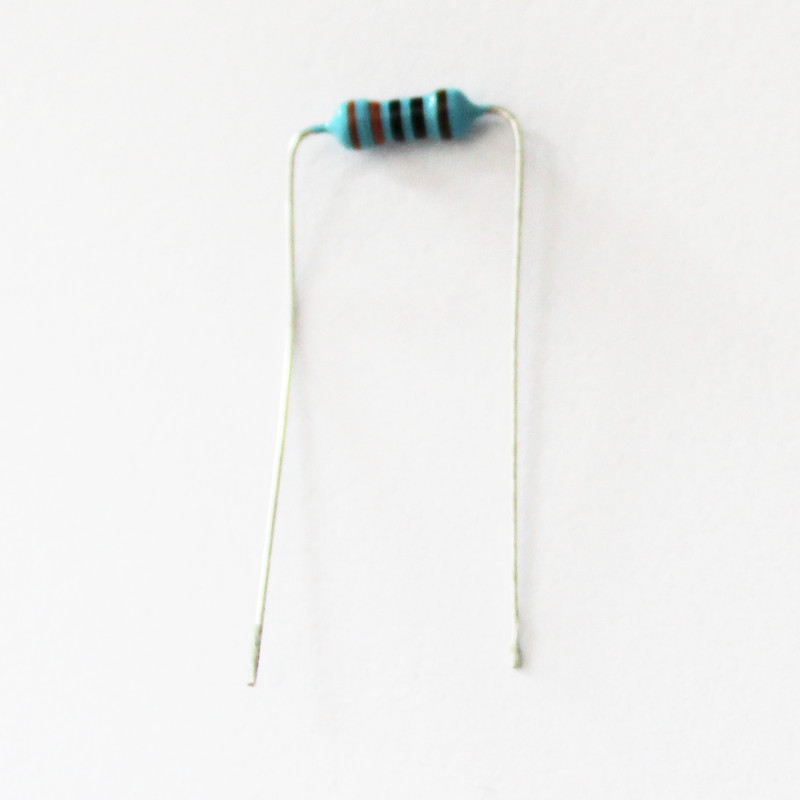
\includegraphics[width=.8\textwidth]{2-hardwaredesign/img/komponenten_elementar_widerstand} \\
        Widerstand

        \column[b]{.25\textwidth}
        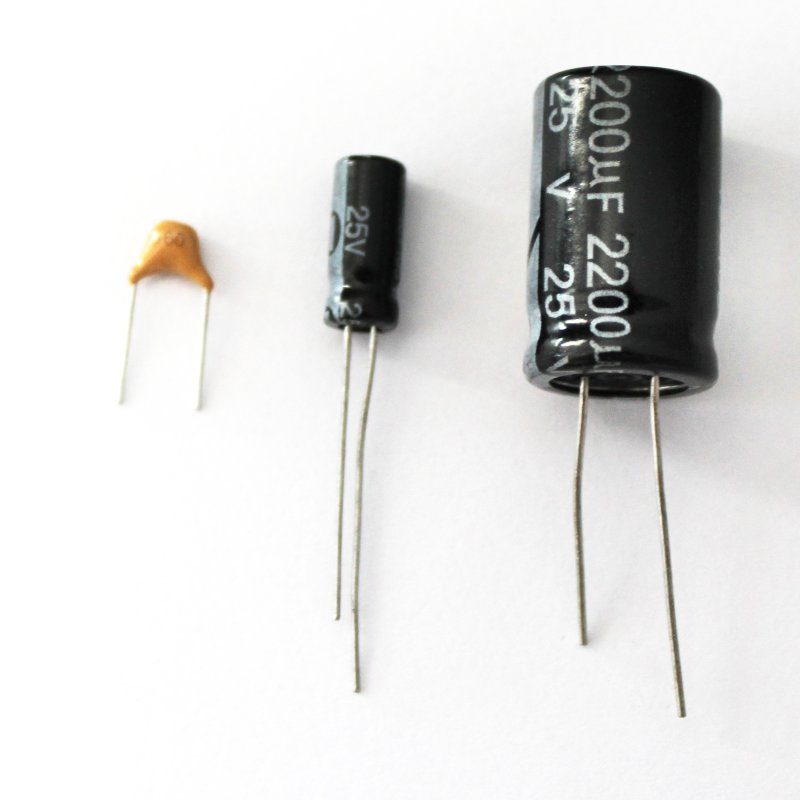
\includegraphics[width=.8\textwidth]{2-hardwaredesign/img/komponenten_elementar_kondensator} \\
        Kondensator

        \column[b]{.25\textwidth}
        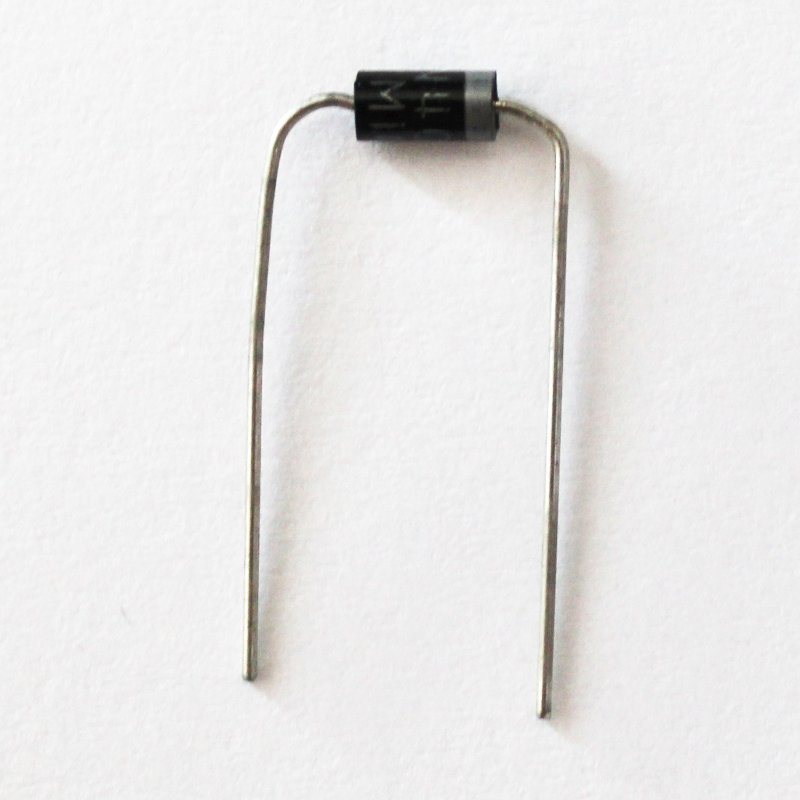
\includegraphics[width=.8\textwidth]{2-hardwaredesign/img/komponenten_elementar_diode} \\
        Diode

        \column[b]{.25\textwidth}
        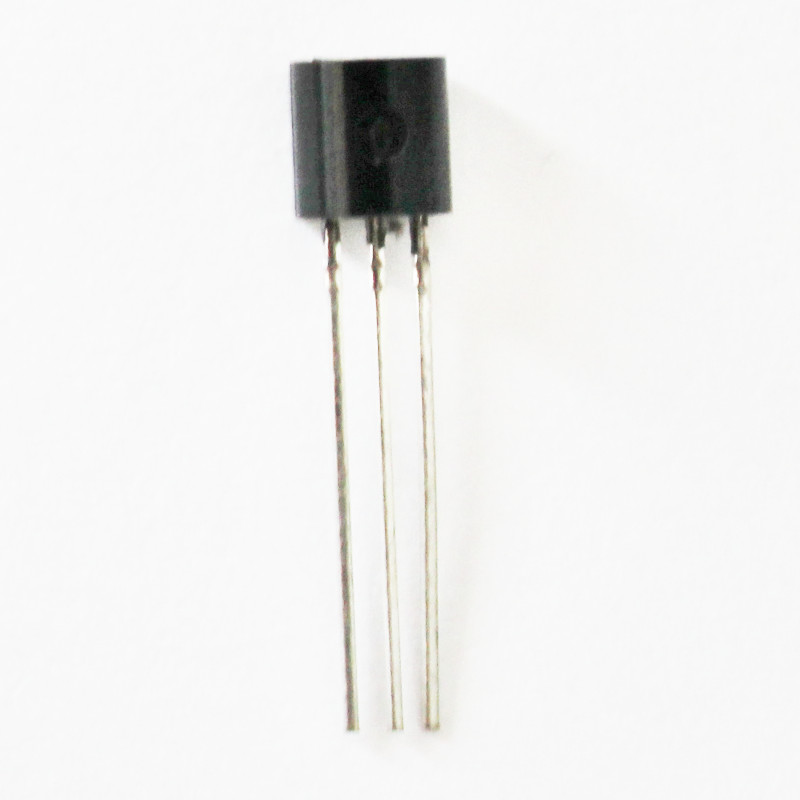
\includegraphics[width=.8\textwidth]{2-hardwaredesign/img/komponenten_elementar_transistor} \\
        Transistor
    \end{columns}

    \bigskip

    \begin{columns}
        \column[b]{.25\textwidth}
        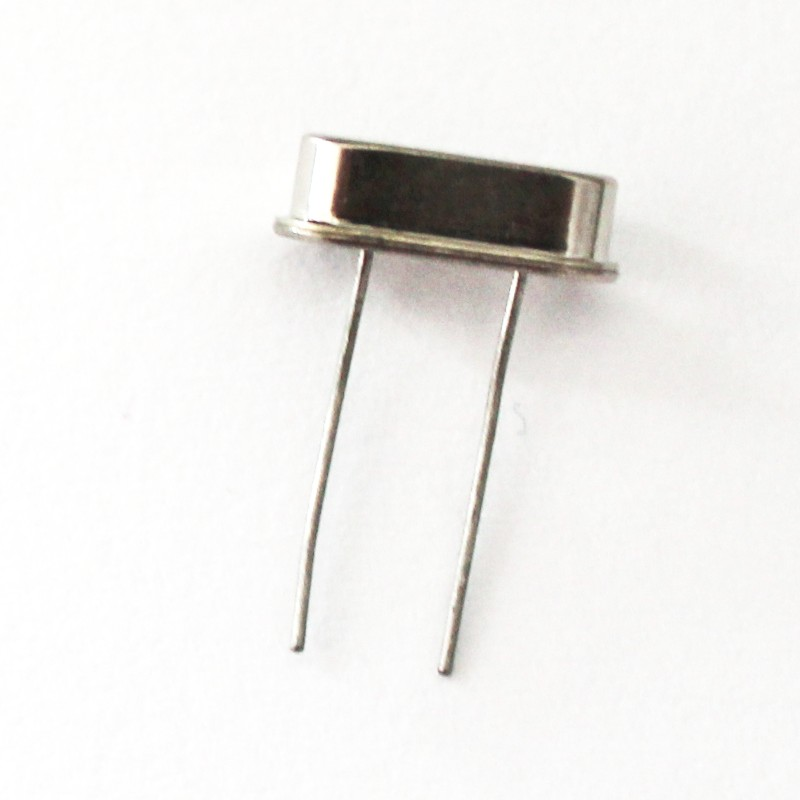
\includegraphics[width=.8\textwidth]{2-hardwaredesign/img/komponenten_elementar_quartz} \\
        Quartz-Kristal

        \column[b]{.25\textwidth}
        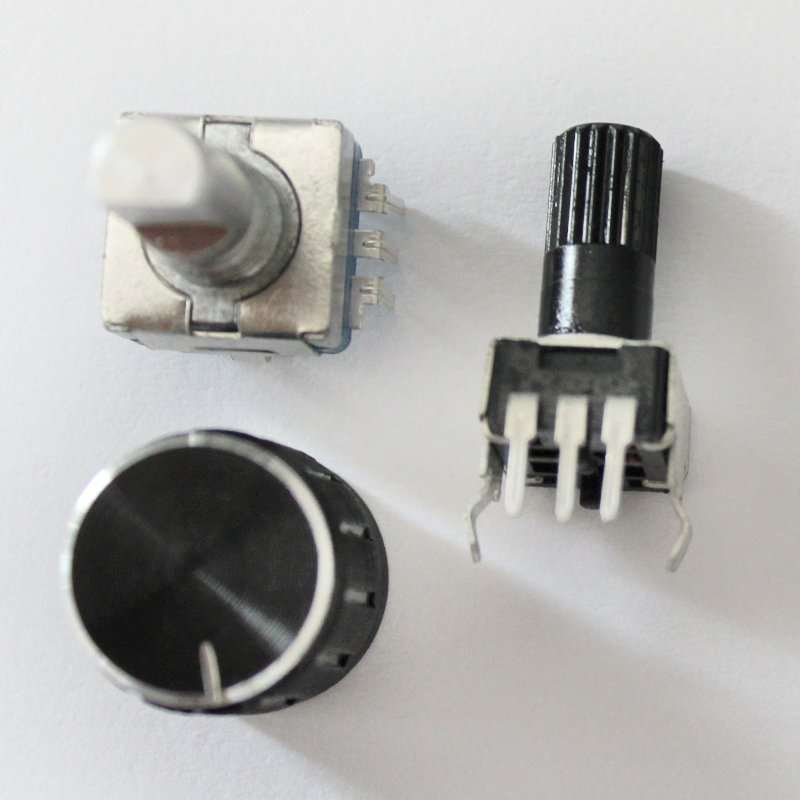
\includegraphics[width=.8\textwidth]{2-hardwaredesign/img/komponenten_elementar_drehregler} \\
        Drehregler

        \column[b]{.25\textwidth}
        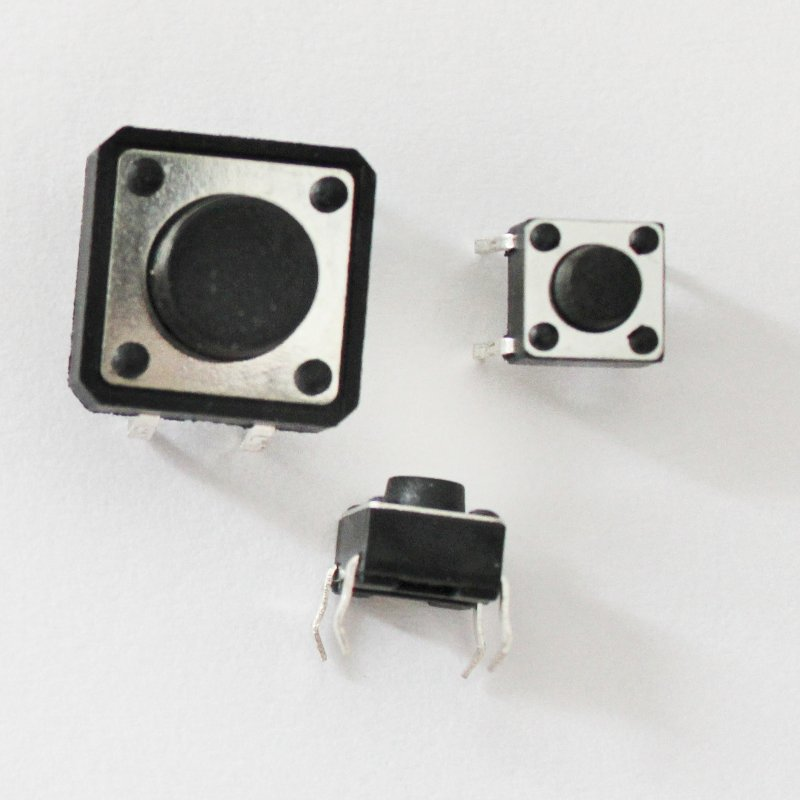
\includegraphics[width=.8\textwidth]{2-hardwaredesign/img/komponenten_elementar_taster} \\
        Taster, Schalter

        \column[b]{.25\textwidth}
        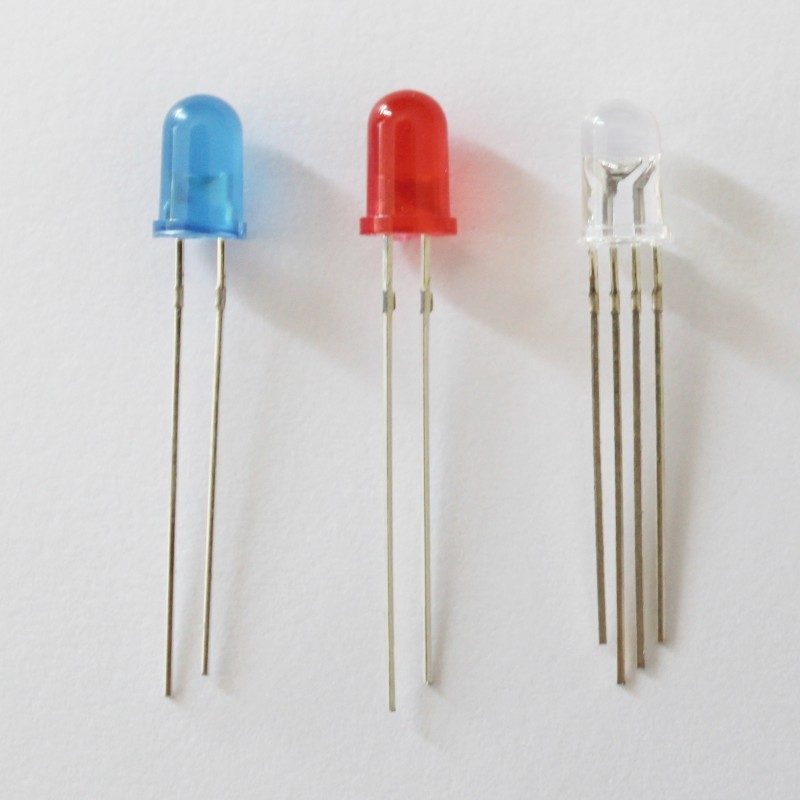
\includegraphics[width=.8\textwidth]{2-hardwaredesign/img/komponenten_elementar_led} \\
        Leuchtdiode
    \end{columns}
\end{frame}
}

%%% Folie
{
\small

\begin{frame}{Beispiel: Integrierte Schaltkreise}
    \begin{columns}
        \column[b]{.5\textwidth}
        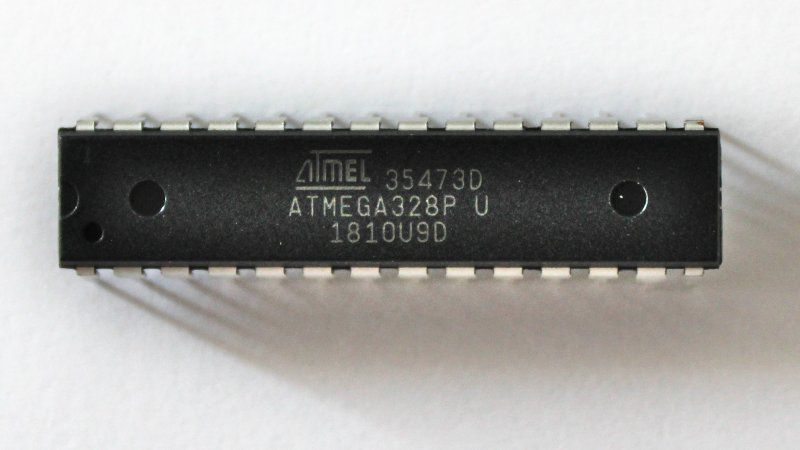
\includegraphics[width=.8\textwidth]{2-hardwaredesign/img/komponenten_ic_prozessor} \\
        Mikroprozessor, Mikrocontroller

        \column[b]{.5\textwidth}
        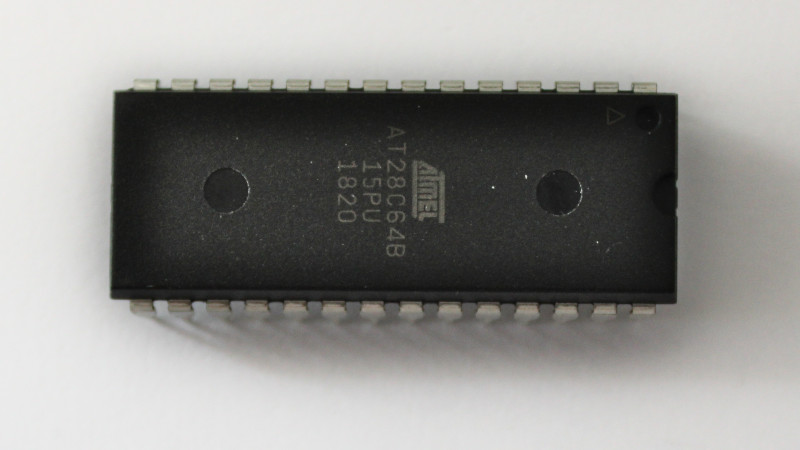
\includegraphics[width=.8\textwidth]{2-hardwaredesign/img/komponenten_ic_speicher} \\
        Speicherbaustein
    \end{columns}

    \bigskip

    \begin{columns}
        \column[b]{.5\textwidth}
        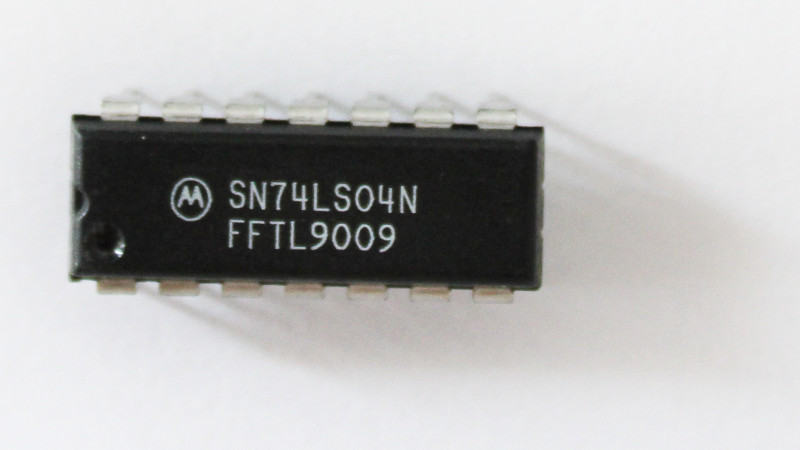
\includegraphics[width=.8\textwidth]{2-hardwaredesign/img/komponenten_ic_logikgatter} \\
        Logikbaustein (AND, OR, XOR, ...)

        \column[b]{.5\textwidth}
        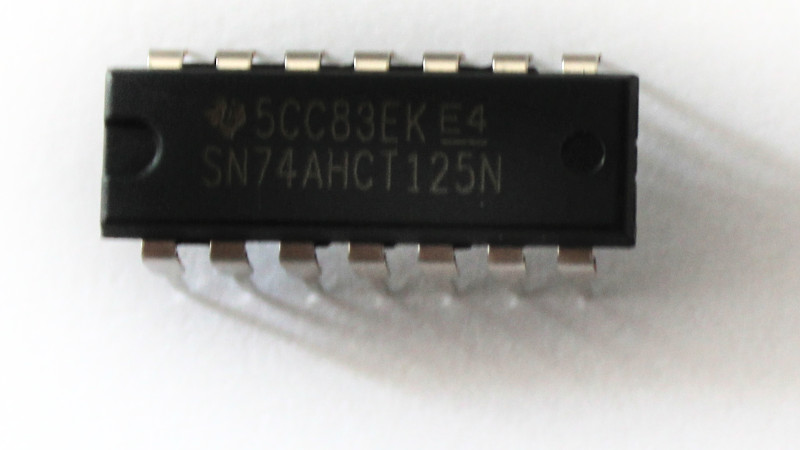
\includegraphics[width=.8\textwidth]{2-hardwaredesign/img/komponenten_ic_levelshifter} \\
        Level Shifter
    \end{columns}
\end{frame}
}

%%% Folie
{
\small

\begin{frame}{Beispiel: Vorgefertigte Baugruppen}
    \begin{columns}
        \column[b]{.5\textwidth}
        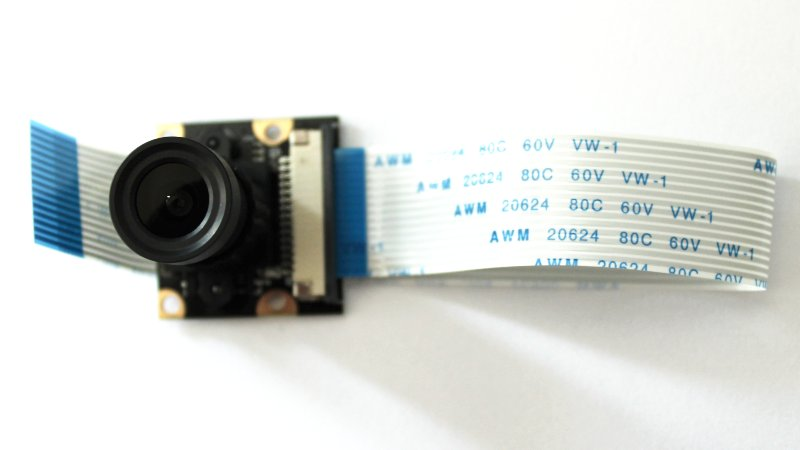
\includegraphics[width=.8\textwidth]{2-hardwaredesign/img/komponenten_baugruppen_kamera} \\
        Kameramodul

        \column[b]{.5\textwidth}
        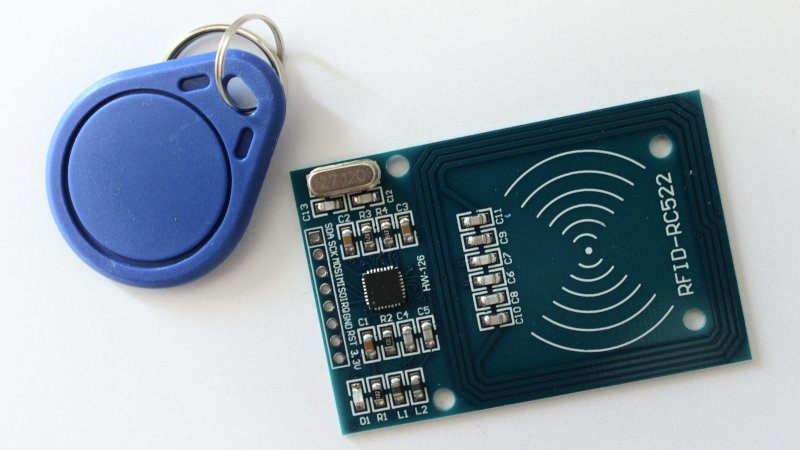
\includegraphics[width=.8\textwidth]{2-hardwaredesign/img/komponenten_baugruppen_rfid} \\
        RFID-Leser
    \end{columns}

    \bigskip

    \begin{columns}
        \column[b]{.5\textwidth}
        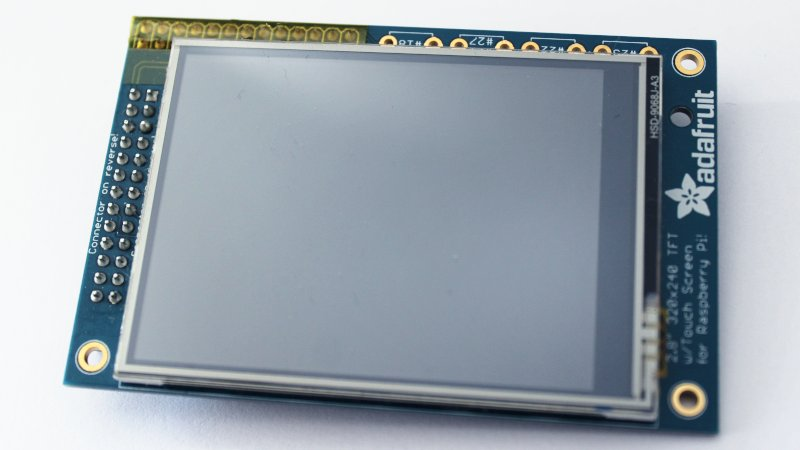
\includegraphics[width=.8\textwidth]{2-hardwaredesign/img/komponenten_baugruppen_display} \\
        Display

        \column[b]{.5\textwidth}
        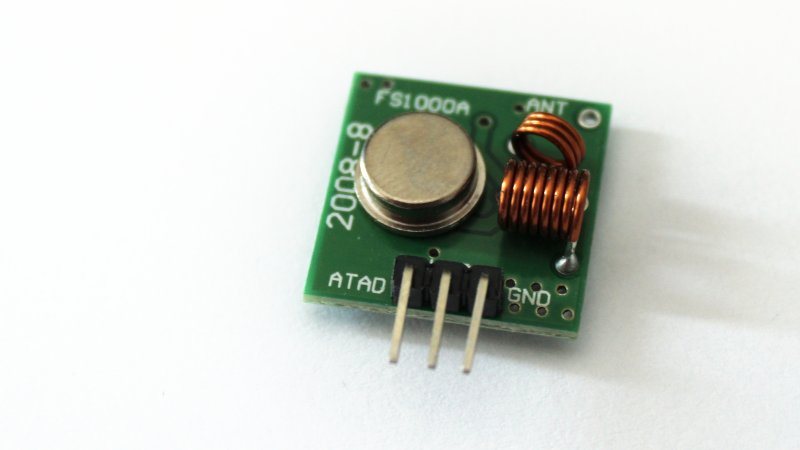
\includegraphics[width=.8\textwidth]{2-hardwaredesign/img/komponenten_baugruppen_funk} \\
        Funkmodul
    \end{columns}
\end{frame}
}

%%% Folie
{
\small

\begin{frame}{Beispiel: Modular einsetzbare Geräte}
    \begin{columns}
        \column[b]{.5\textwidth}
        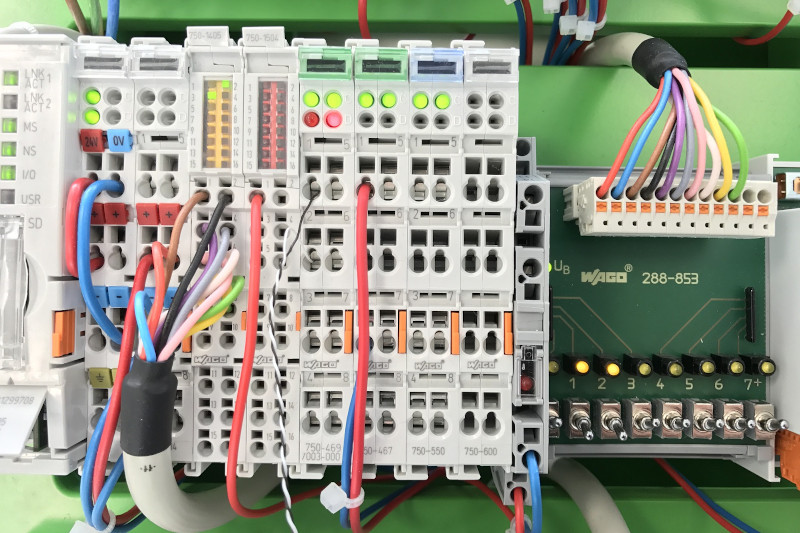
\includegraphics[width=.8\textwidth]{2-hardwaredesign/img/komponenten_geraete_industriesteuerung} \\
        Industrielle Steuergeräte

        \column[b]{.5\textwidth}
        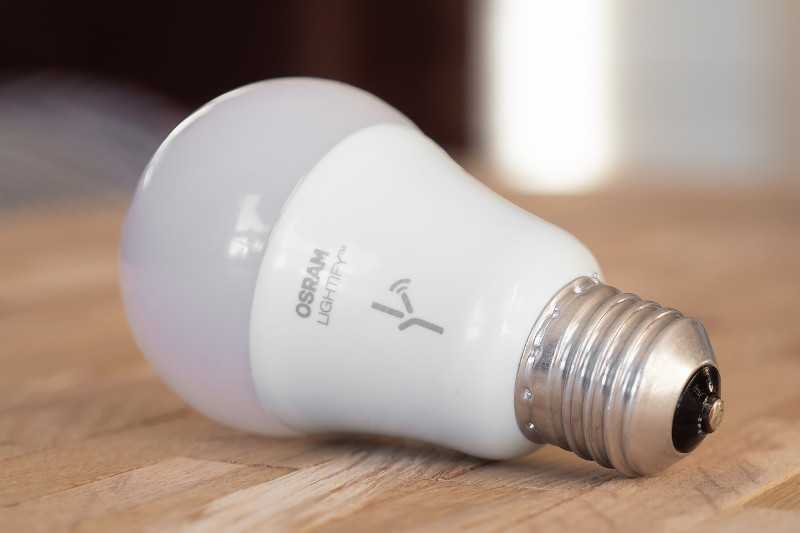
\includegraphics[width=.8\textwidth]{2-hardwaredesign/img/komponenten_geraete_smarthome} \\
        Smart-Home-Komponenten
    \end{columns}

    \bigskip

    \begin{columns}
        \column[b]{.5\textwidth}
        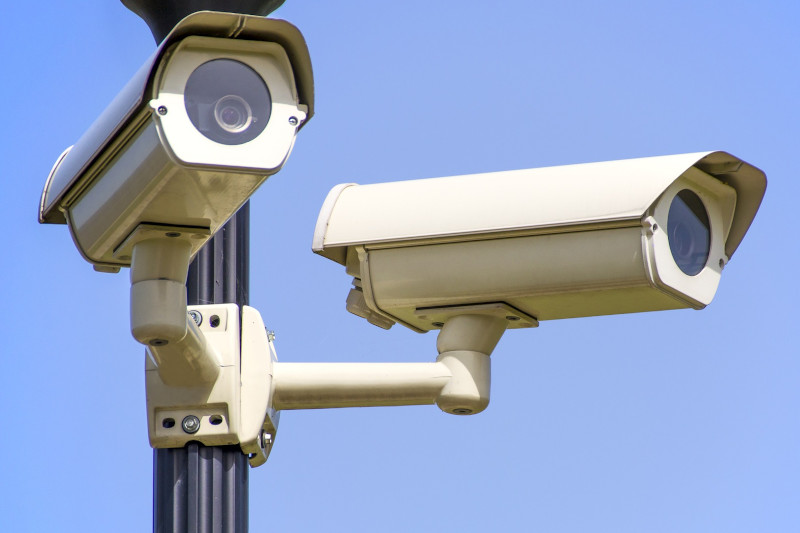
\includegraphics[width=.8\textwidth]{2-hardwaredesign/img/komponenten_geraete_ipkamera} \\
        IP-Kameras

        \column[b]{.5\textwidth}
        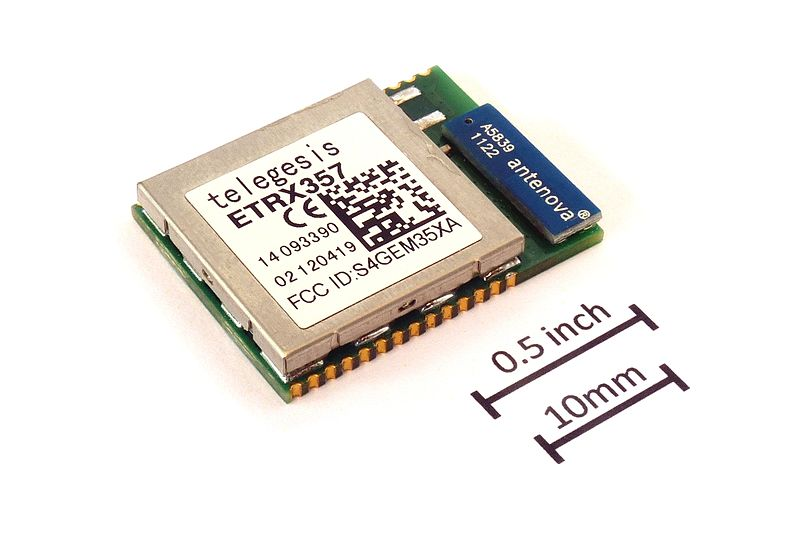
\includegraphics[width=.8\textwidth]{2-hardwaredesign/img/komponenten_geraete_zigbee} \\
        ZigBee-Sensoren und Aktoren
    \end{columns}
\end{frame}
}

%%% Folie
\begin{frame}{Anschlüsse am Raspberry Pi}
        \begin{center}
            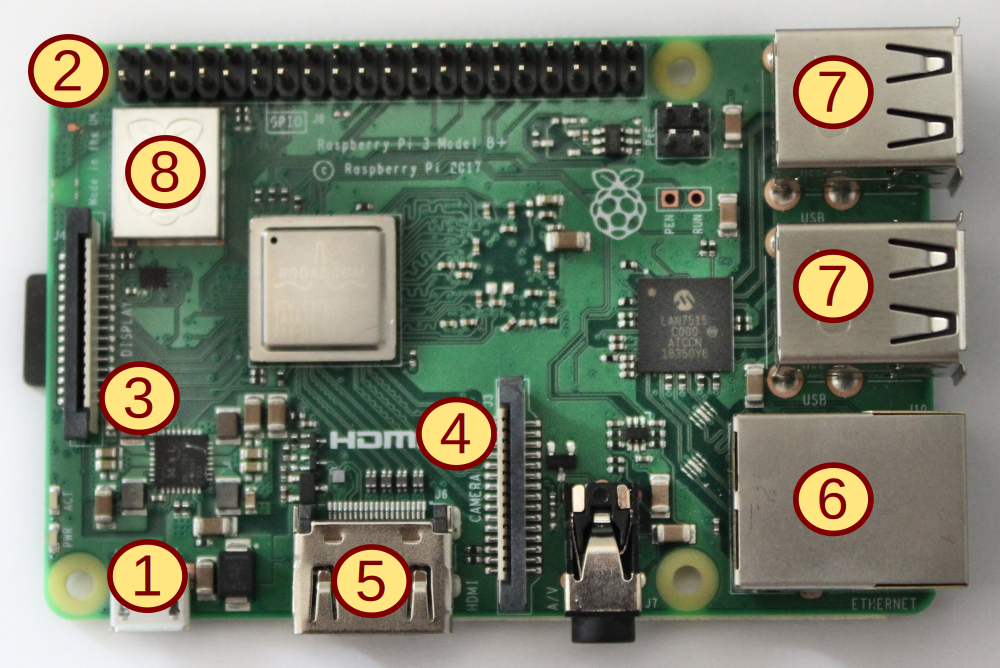
\includegraphics[height=0.5\textheight]{2-hardwaredesign/img/raspberry_anschluesse}
        \end{center}

        \smallskip

        \begin{columns}
            \begin{column}[T]{.5\textwidth}
                \begin{enumerate}
                    \item Mini-USB Stromversorgung
                    \item J8 GPIO-Header
                    \item Display Serial Interface
                    \item Camera Serial Interface
                \end{enumerate}
            \end{column}
            \begin{column}[T]{.5\textwidth}
                \begin{enumerate}
                    \setcounter{enumi}{4}   % Zielwert - 1
                    \item HDMI-Bildschirmanschluss
                    \item LAN-Netzwerkanschluss
                    \item USB (4 Stück)
                    \item WiFi, Bluetooth
                \end{enumerate}
            \end{column}
        \end{columns}
\end{frame}

%%% Folie
{
\footnotesize

\begin{frame}{Der J8 GPIO-Header im Detail}
        \begin{columns}
            \column[b]{.5\textwidth}
            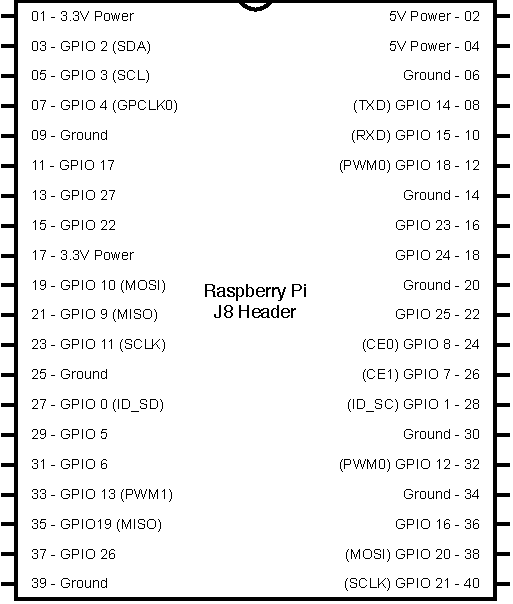
\includegraphics[width=\textwidth]{2-hardwaredesign/img/raspberry_j8}

            \column[b]{.5\textwidth}
            \begin{block}{Stromquellen}
                \begin{itemize}
                    \item 5V Power
                    \item 3.3V Power
                    \item Ground (Masse)
                \end{itemize}
            \end{block}

            \begin{block}{Digitale Ein-/Ausgänge}
                \begin{itemize}
                    \item GPIO
                    \item Pulsweitenmodulation
                    \item Asynchron serielle Kommunikation
                    \item Synchron serielle Kommunikation \\ (SPI, I²C, I²S, 1-Wire)
                \end{itemize}
            \end{block}

            \begin{alertblock}{Keine analogen Ein-/Ausgänge!}
            \end{alertblock}
        \end{columns}
\end{frame}
}

%%% Folie
{
    \setbeamertemplate{background canvas}{
        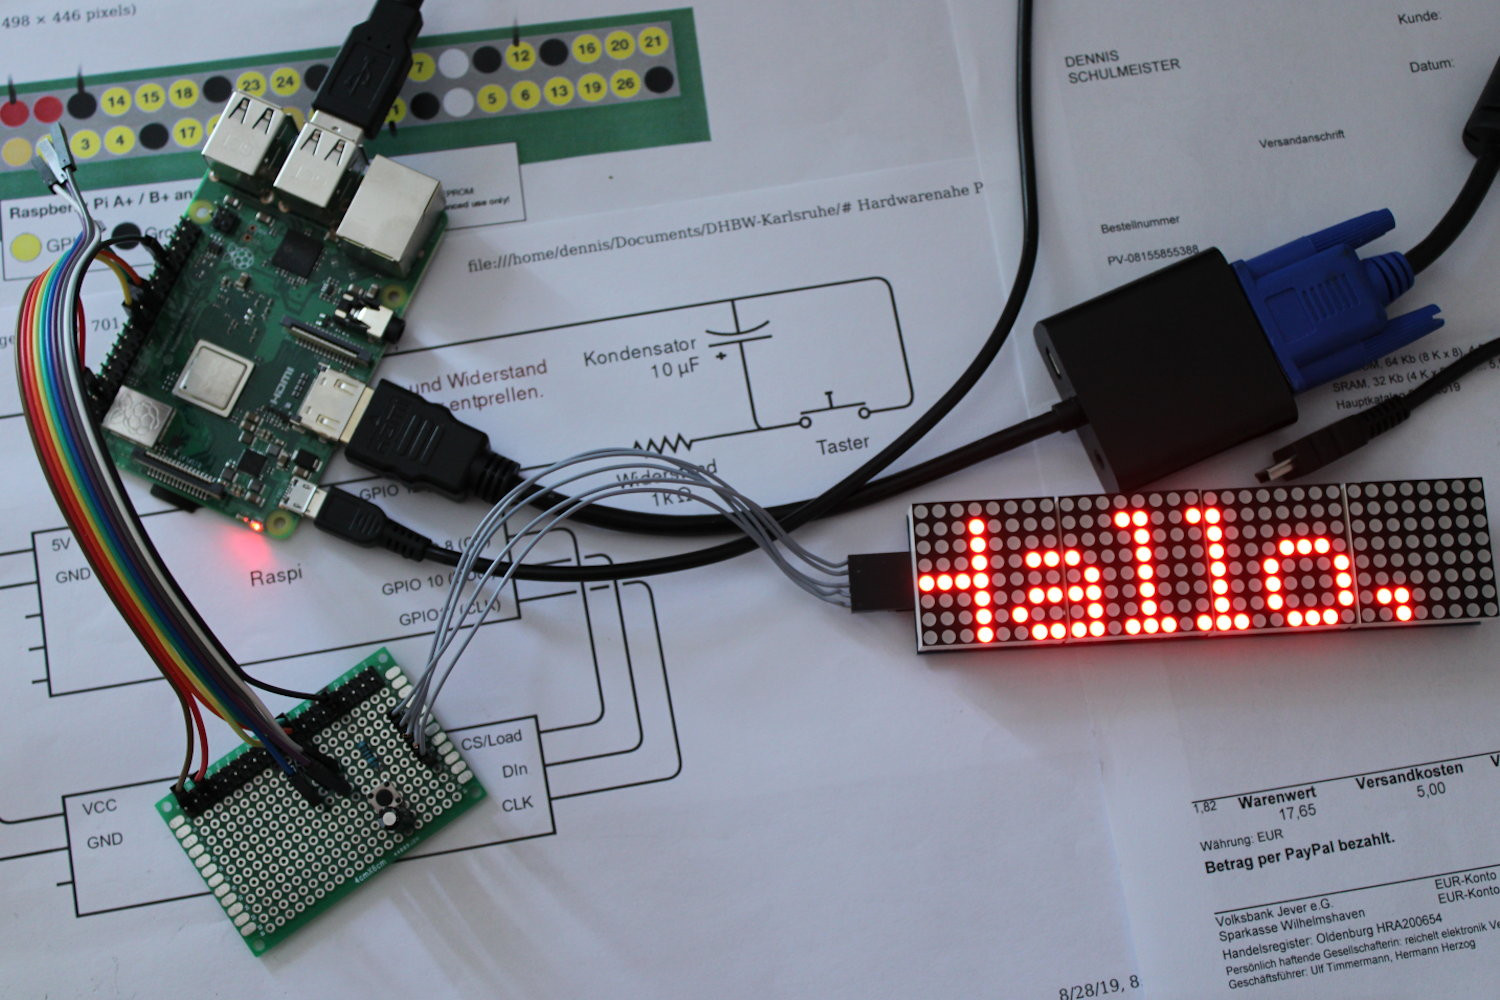
\includegraphics[height=\paperheight, width=\paperwidth]{2-hardwaredesign/img/vorgehen_lochrasterplatine}
    }

    \begin{frame}[plain]
    \end{frame}
}

%-------------------------------------------------------------------------------
\section{Elektronik-Grundwissen}
%-------------------------------------------------------------------------------

%%% Folie
\begin{frame}{Vom Atom zur Ladung zur Spannung}
    \begin{columns}
        \column{.6\textwidth}
        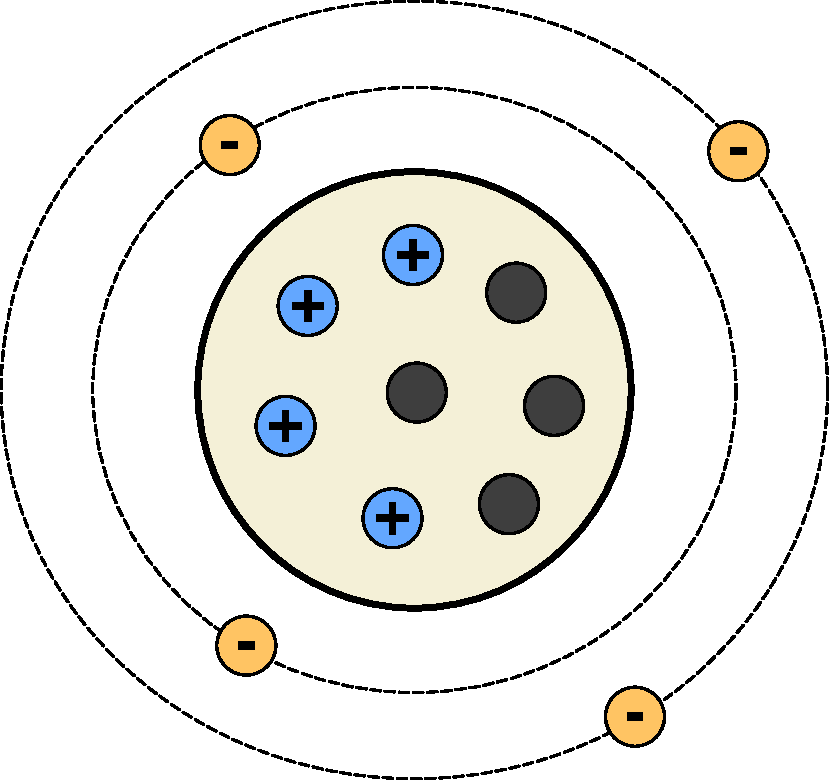
\includegraphics[width=.8\textwidth]{2-hardwaredesign/img/atom_detail}

        \column{.4\textwidth}
        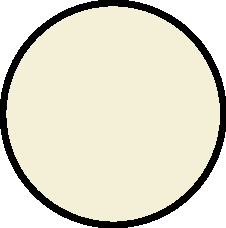
\includegraphics[width=.5cm]{2-hardwaredesign/img/atom_kern}
        \hskip 1em
        Atomkern \\
        \smallskip

        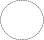
\includegraphics[width=.5cm]{2-hardwaredesign/img/atom_schale}
        \hskip 1em
        Schale \\
        \bigskip

        
\includegraphics[width=.5cm]{2-hardwaredesign/img/atom_elektron}
        \hskip 1em
        Elektron \\
        \smallskip

        
\includegraphics[width=.5cm]{2-hardwaredesign/img/atom_proton}
        \hskip 1em
        Proton \\
        \smallskip

        
\includegraphics[width=.5cm]{2-hardwaredesign/img/atom_neutron}
        \hskip 1em
        Neutron \\
    \end{columns}

    \bigskip
    \bigskip

    \parbox{\linewidth}{
        \footnotesize
        Atome sind im Normalzustand elektrisch neutral, da sie die gleiche Anzahl
        Protonen wie Elektronen besitzen. Atome mit einem Überschuss oder Mangel
        an Elektronen werden \glqq{}Ionen\grqq{} genannt und sind \glqq{}elektrisch
        geladen\grqq{}. Misst man die Ladungsdifferenz an zwei Punkten, erhält man
        die \glqq{}Spannung\grqq{}, welche als Kraft auf die Elektronen einwirkt.
    }
\end{frame}

%%% Folie
\begin{frame}{Spannung liegt an, Strom fließt}
    \begin{columns}
        \column{\dimexpr\paperwidth-28pt}
        \begin{center}
            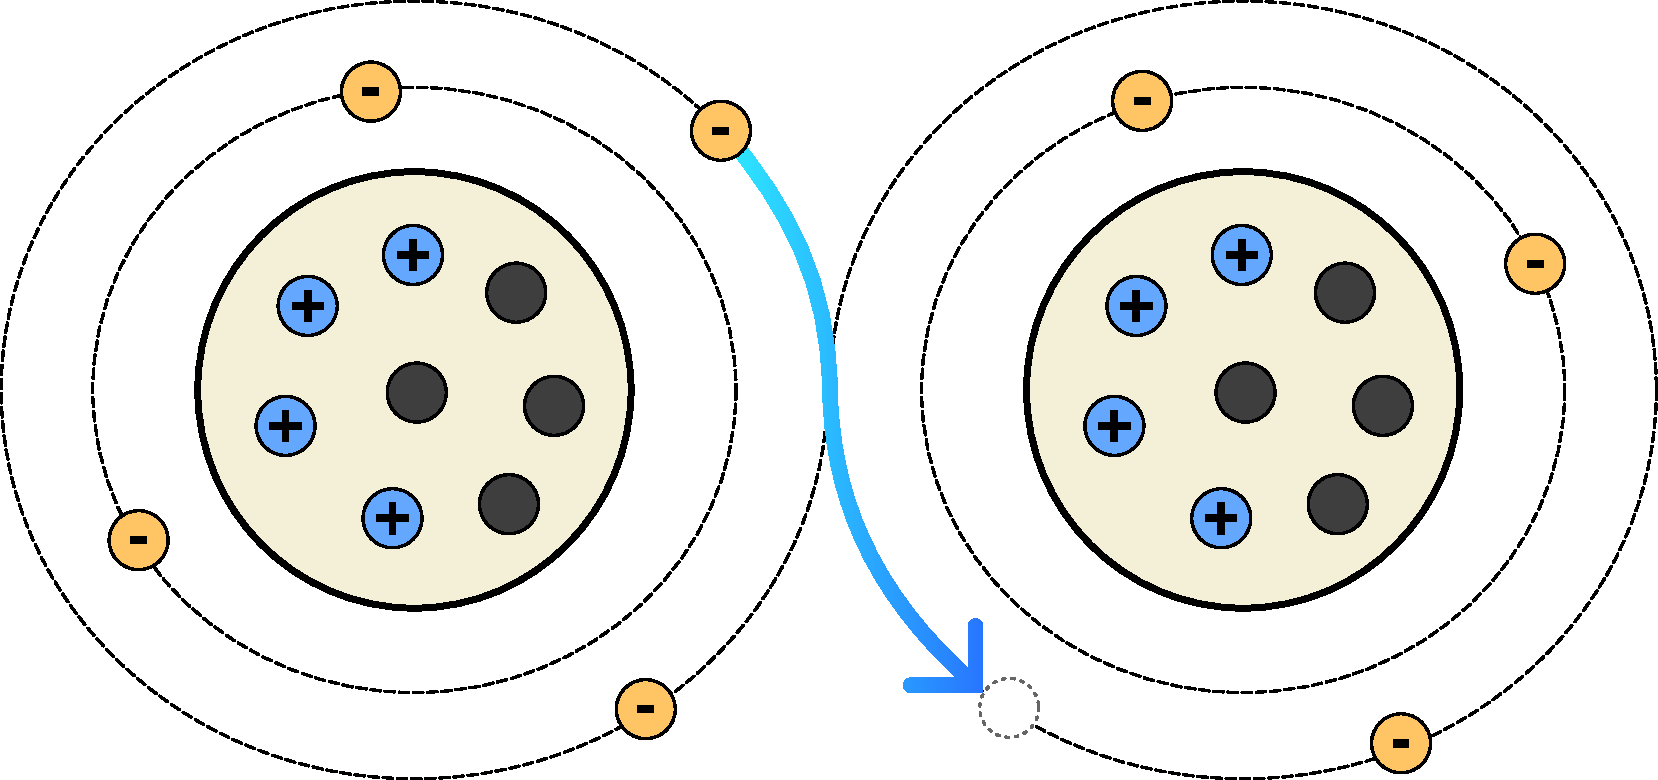
\includegraphics[width=.9\textwidth]{2-hardwaredesign/img/atom_elektronenfluss}
        \end{center}
    \end{columns}

    \bigskip

    \parbox{\linewidth}{
        \footnotesize
        In festen Stoffen fließt Strom, indem die freien Valenzelektronen der Atome
        bewegt werden. Ausgehend von einem negativ geladenen Pol mit Eletrkonenüberschuss
        laufen die Elektronen dabei hin zum positiven Pol mit Elektronenmangel und
        verrichten dadurch Arbeit. Die Flussgeschwindigkeit nennt man \glqq{}Stromstärke\grqq{}.
    }
\end{frame}

%%% Folie
\begin{frame}{Maßeinheiten und Größen}
    \begin{tabularx}{\textwidth}{|X|X|X|}
        \hline
        \textbf{Präfix} & \textbf{Zehnerpotenz} & \textbf{Dezimalwert} \\
        \hline

        Mega & $10^6$ & 1.000.000 \\
        \hline

        Kilo & $10^3$ & 1.000 \\
        \hline

        -- & $10^0$ & 1 \\
        \hline

        Milli & $10^{-3}$ & 0,01 \\
        \hline

        Mikro & $10^{-6}$ & 0,00.001 \\
        \hline

        Nano & $10^{-9}$ & 0,00.000.001 \\
        \hline

        Piko & $10^{-12}$ & 0,00.000.000.001 \\
        \hline
    \end{tabularx}

    \bigskip
    \bigskip
    \bigskip

    {
        \small

        \textbf{Spannung:} Volt \hskip 1em
        \textbf{Stromstärke:} Ampere \hskip 1em
        \textbf{Widerstand:} Ohm \hskip 1em
        \textbf{Leistung:} Watt
    }
\end{frame}

%%% Folie
\begin{frame}{Das Ohmsche Gesetz}
    \begin{columns}
        \column{0.4\textwidth}
        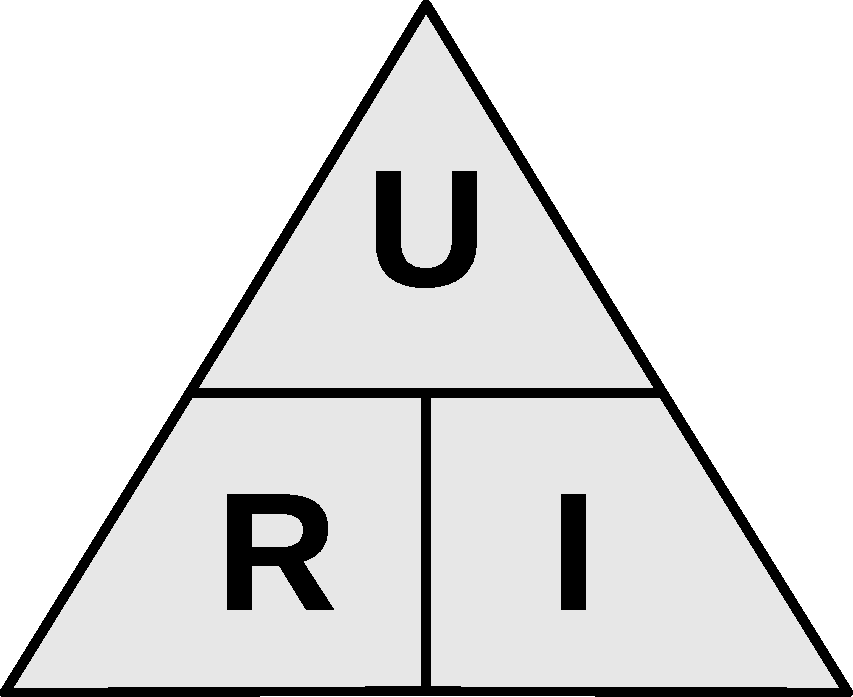
\includegraphics[width=.5\textwidth]{2-hardwaredesign/img/formel_uri}

        \bigskip

        $U = R * I$ \\
        \smallskip
        $R = U / I$ \\
        \smallskip
        $I = U / R$ \\

        \bigskip
        {
            \footnotesize
            \textbf{R}: Widerstand in Ohm \\
            \smallskip
            \textbf{U}: Spannung in Volt \\
        }

        \column{0.4\textwidth}
        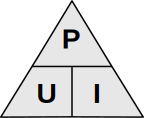
\includegraphics[width=.5\textwidth]{2-hardwaredesign/img/formel_pui}

        \bigskip

        $P = U * I$ \\
        \smallskip
        $U = P / I$ \\
        \smallskip
        $I = P / U$ \\

        \bigskip
        {
            \footnotesize
            \textbf{I}: Stromstärke in Ampere\\
            \smallskip
            \textbf{P}: Leistung in Watt \\
        }
    \end{columns}

    \bigskip

    \parbox{\linewidth}{
        \footnotesize
        Spannung, Stromstärke, Widerstand und Leistung stehen immer in Zusammenhang,
        so dass man anhand von zwei Werten die beiden anderen berechnen kann.
        Die hier gezeigten Formeln gelten allerdings nur für \textbf{ohmsche Widerstände}
        mit linearem Zusammenhang zwischen Spannung und Stromstärke. Viele gängige Bauteile
        wie z.B.\,LEDs haben allerdings eine nicht-lineare Kennlinie!
    }
\end{frame}

%%% Folie
{
\small

\begin{frame}{In Reihe geschaltete Widerstände: Spannungsteiler}
    \begin{columns}
        \column{0.7\textwidth}
        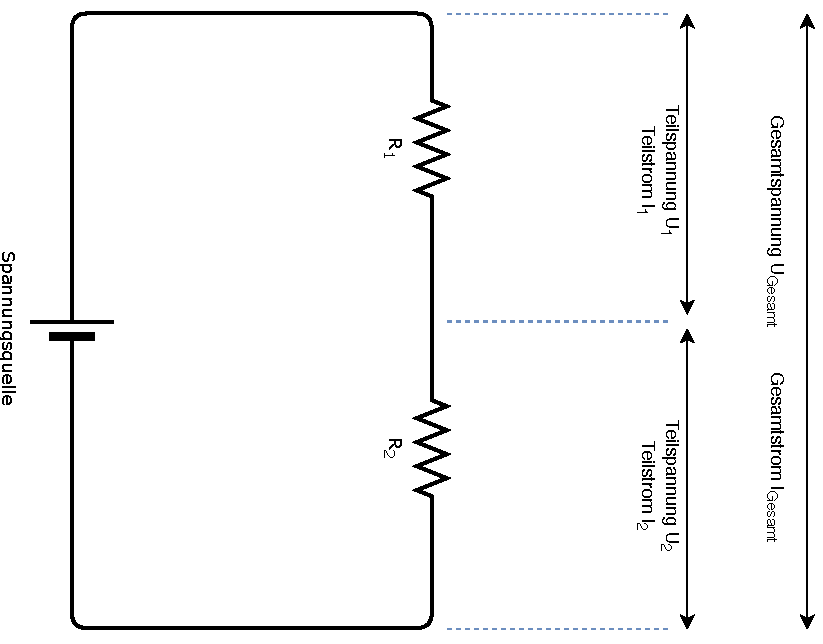
\includegraphics[width=\textwidth]{2-hardwaredesign/img/spannungsteiler}

        \column{0.3\textwidth}
        In Reihe geschaltete Widerstände teilen die Spannung.
        Es kommt zum \textbf{Spannungsabfall}.

        \bigskip
        \bigskip

        $R_{Gesamt} = R_1 + R_2$ \\
        \smallskip
        $U_{Gesamt} = U_1 + U_2$ \\
        \smallskip
        $U_1 / U_2 = R_1 / R_2$ \\
        \smallskip
        $I_{Gesamt} = I_1 = I_2$ \\

        \bigskip
        \bigskip

        \textbf{R}: Widerstand in Ohm \\
        \smallskip
        \textbf{U}: Spannung in Volt \\
        \smallskip
        \textbf{I}: Stromstärke in Ampere \\
    \end{columns}
\end{frame}
}

%%% Folie
{
\small

\begin{frame}{Parallel geschaltete Widerstände: Stromteiler}
    \begin{columns}
        \column{0.7\textwidth}
        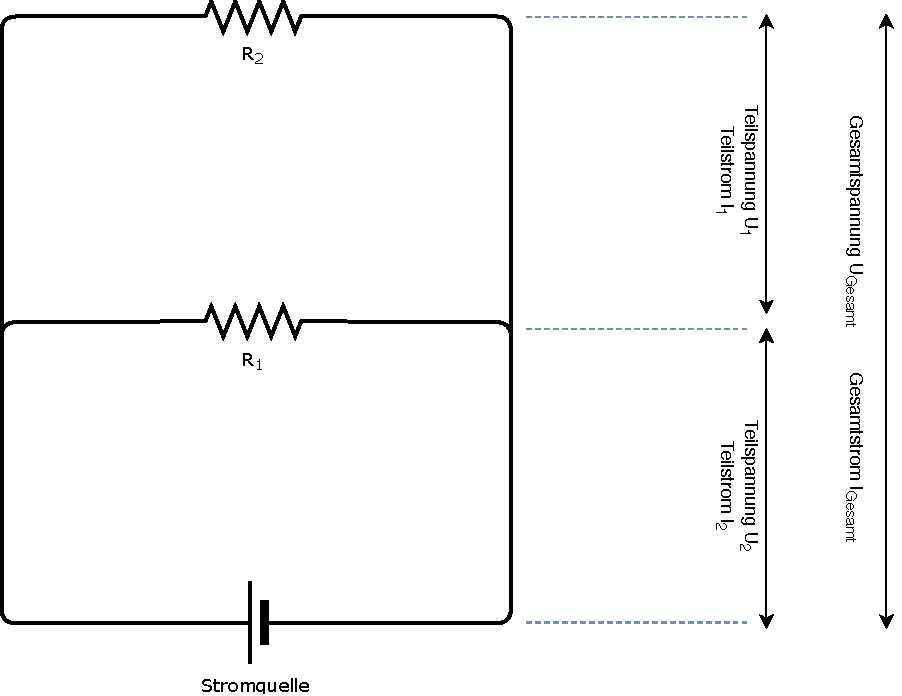
\includegraphics[width=\textwidth]{2-hardwaredesign/img/stromteiler}

        \column{0.3\textwidth}
        Parallel geschaltete Widerstände teilen die Stromstärke.
        Es kommt zum \textbf{Stromabfall}.

        \bigskip
        \bigskip

        $1/R_{Gesamt} = 1/R_1 + 1/R_2$ \\
        \smallskip
        $U_{Gesamt} = U_1 = U_2$ \\
        \smallskip
        $I_1 / I_2 = R_1 / R_2$ \\
        \smallskip
        $I_{Gesamt} = I_1 + I_2$ \\

        \bigskip
        \bigskip

        \textbf{R}: Widerstand in Ohm \\
        \smallskip
        \textbf{U}: Spannung in Volt \\
        \smallskip
        \textbf{I}: Stromstärke in Ampere \\
    \end{columns}
\end{frame}
}


%-------------------------------------------------------------------------------
\section{Grundschaltungen einfacher µC-Anwendungen}
%-------------------------------------------------------------------------------

%%% Folie
\begin{frame}[allowframebreaks]{Vorgehen bei der Entwicklung einer neuen Schaltung}
    \begin{enumerate}
        \item Definition der zu erfüllenden Anforderungen
        \item Anfertigen einer groben Hardwareskizze
        \item Passende Bauelemente suchen und beschaffen
        \item Datenblätter studieren, studieren, studieren, ...
        \item Schaltplan Schritt für Schritt ausarbeiten
        \item Firmware entwickeln
        \item Schaltung auf Breadboard/Lochrasterplatine testen
        \item Leiterplatte entwerfen und fertigen (lassen)
    \end{enumerate}

    \begin{columns}
        \column{0.5\textwidth}
        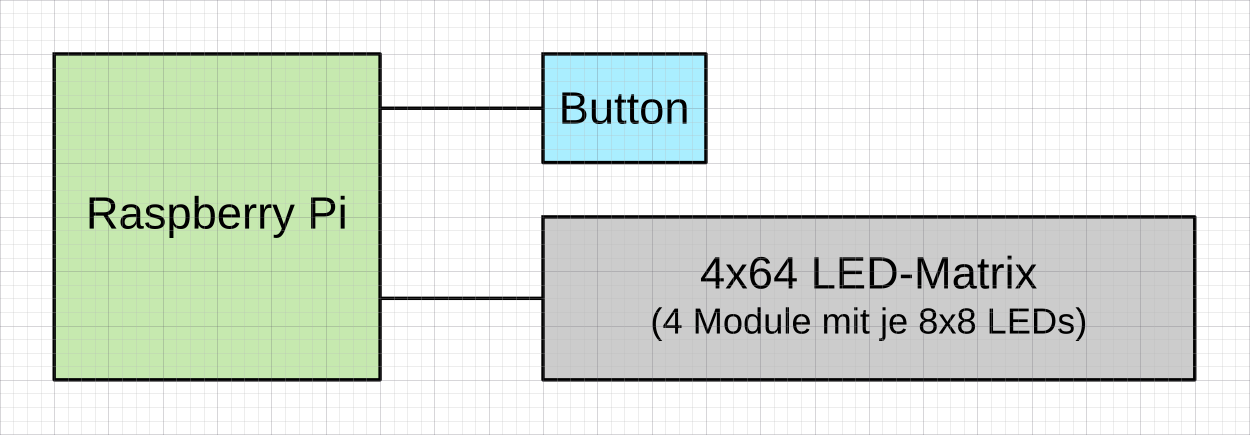
\includegraphics[width=\textwidth]{2-hardwaredesign/img/vorgehen_skizze}

        \column{0.5\textwidth}
        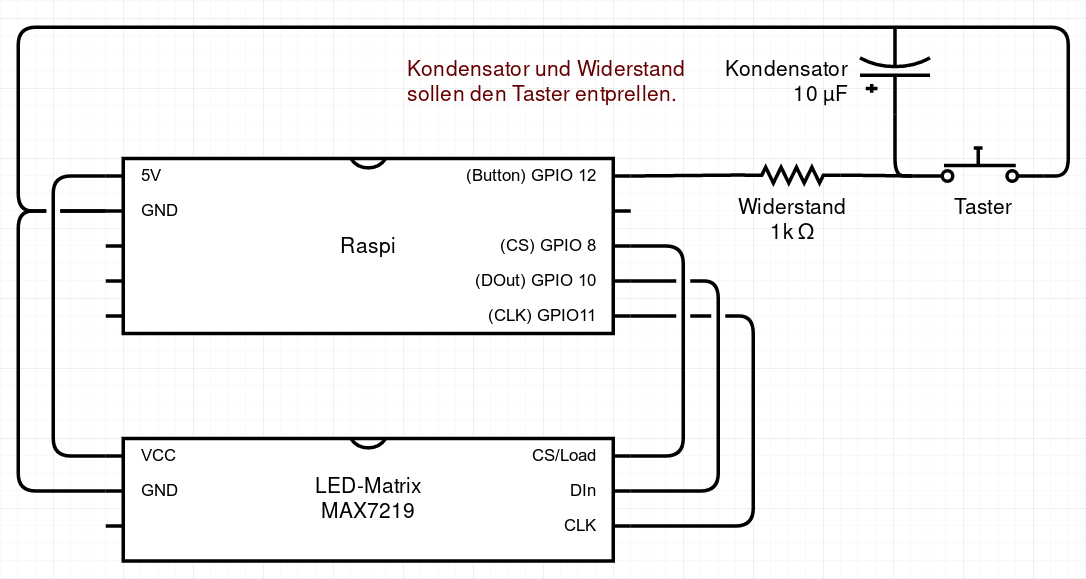
\includegraphics[width=\textwidth]{2-hardwaredesign/img/vorgehen_schaltplan}
    \end{columns}

    \bigskip

    \begin{columns}
        \column{0.5\textwidth}
        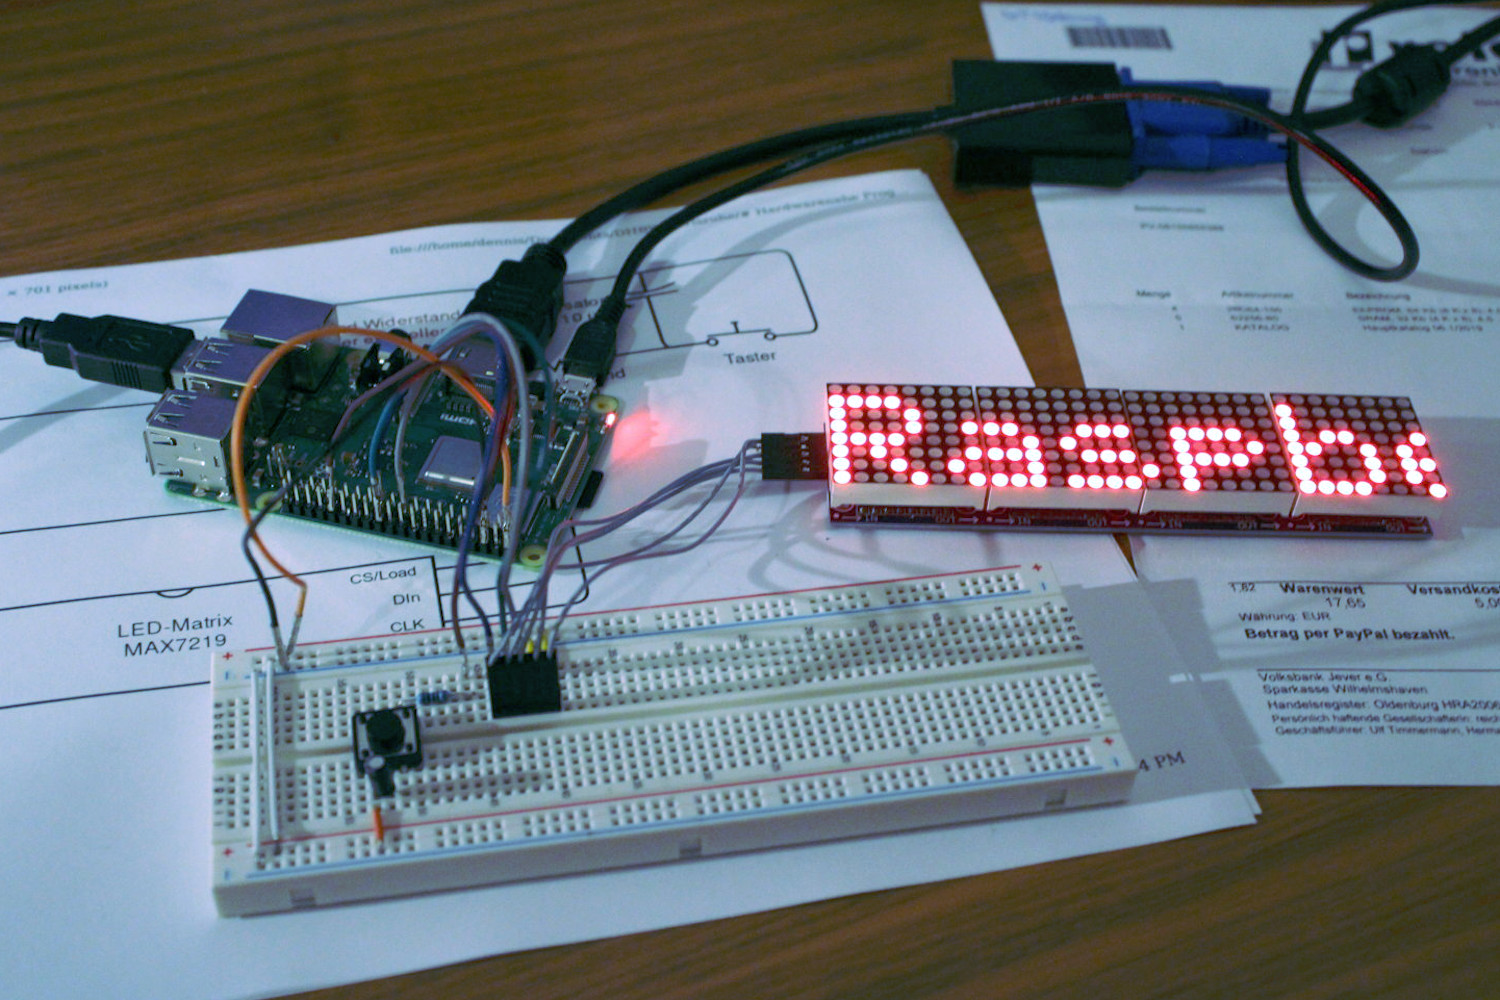
\includegraphics[width=\textwidth]{2-hardwaredesign/img/vorgehen_breadboard}

        \column{0.5\textwidth}
        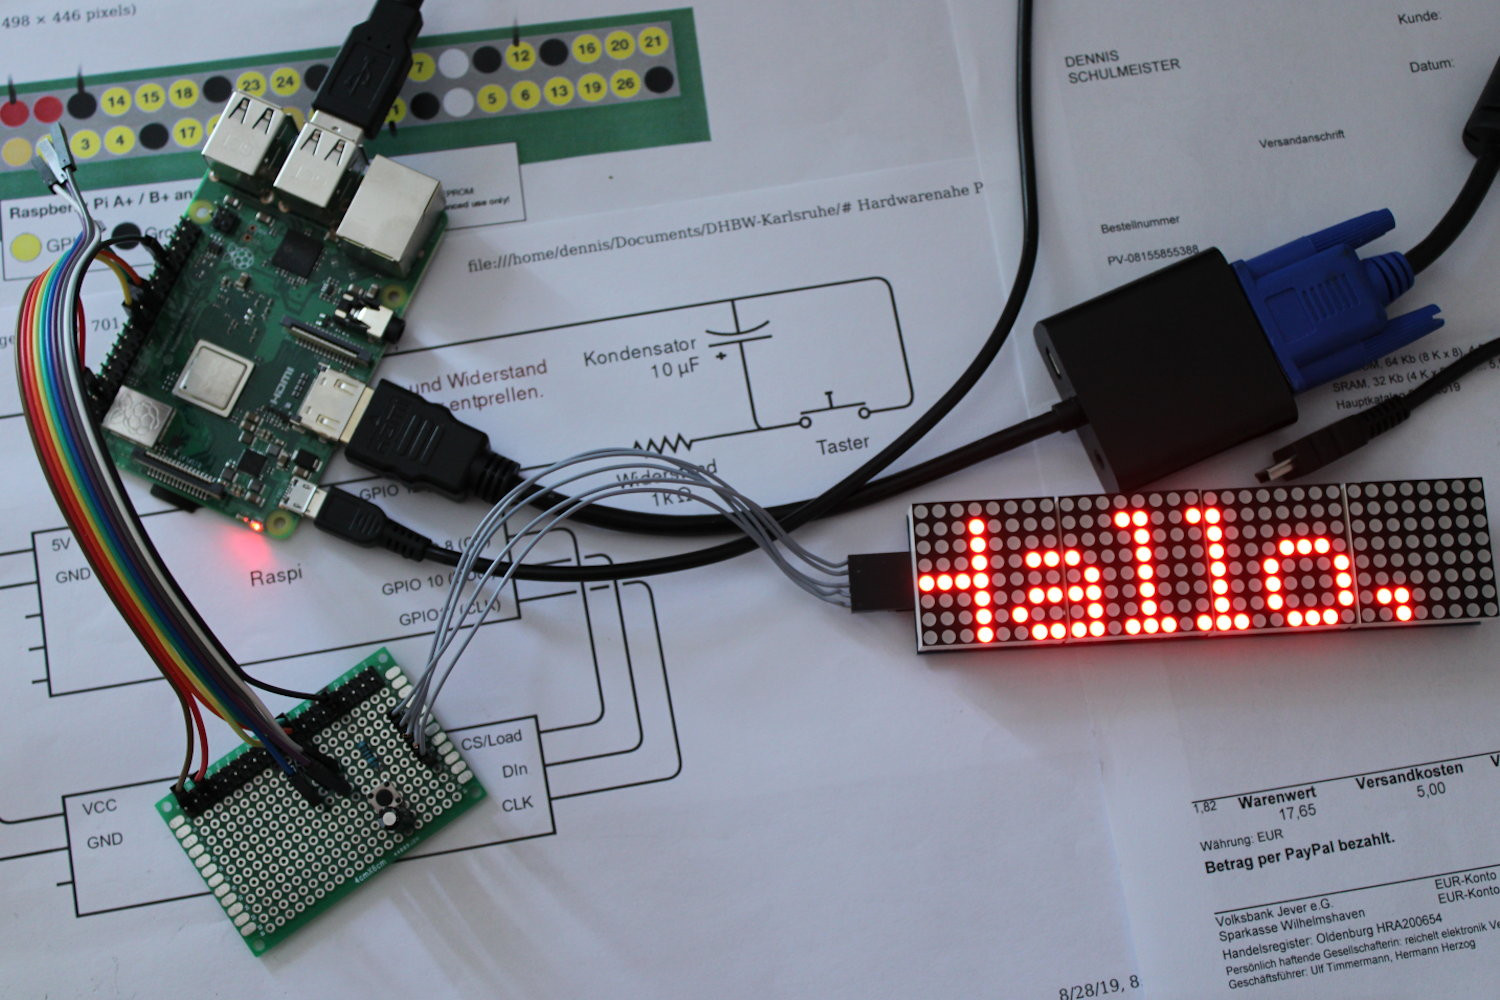
\includegraphics[width=\textwidth]{2-hardwaredesign/img/vorgehen_lochrasterplatine}
    \end{columns}
\end{frame}

%%% Folie
{
\small

\begin{frame}{Bevor es losgehen kann: Maximale Grenzwerte}
    \parbox{\linewidth}{
        Um eine Beschädigung des Raspberry Pi zu vermeiden, müssen folgende Grenzwerte unbedingt
        eingehalten werden. Bei der Berechnung hilft uns das eben kennengelernte ohmsche Gesetz.
    }

    \bigskip

    \begin{tabularx}{\textwidth}{|X|X|X|}
        \hline
        \textbf{Parameter} & \textbf{Mindestwert} & \textbf{Maximalwert} \\
        \hline

        Betriebsspannung des Pi & 5\,V & 5\,V \\
        \hline

        Stromverbrauch des Pi & 400 bis 690\,mA & je nach angeschlossenen Verbrauchern \\
        \hline

        Stromentnahme an den 3.3\,V-Pins & -- & 50\,mA gesamt \\
        \hline

        Stromentnahme an den 5\,V-Pins & -- & 50\,mA gesamt \\
        \hline

        Stromentnahme an einem GPIO-Pin & -- & 16\,mA \\
        \hline

        Stromentnahme an allen GPIO-Pins & -- & 50\,mA gesamt \\
        \hline
    \end{tabularx}
\end{frame}
}

%%% Folie
{
\footnotesize

\begin{frame}{LED über Widerstand direkt ansteuern}
    \parbox{\linewidth}{
        Der \textbf{Widerstand} begrenzt den Strom, der durch den Verbraucher (hier die LED)
        fließt. Generell eine gute Idee, jedoch können die Ausgangs-Pins des Raspberry Pi,
        wie eben dargestellt, nur ganz kleine Lasten bewerkstelligen.
    }

    \bigskip

    \begin{columns}
        \column{0.5\textwidth}
        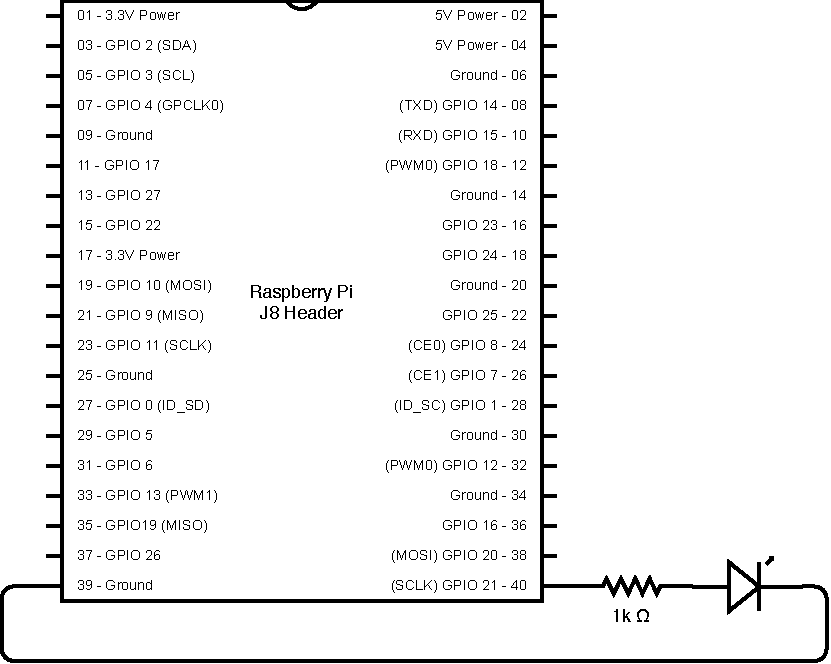
\includegraphics[width=\textwidth]{2-hardwaredesign/img/led_direkt_schaltplan}

        \column{0.5\textwidth}
        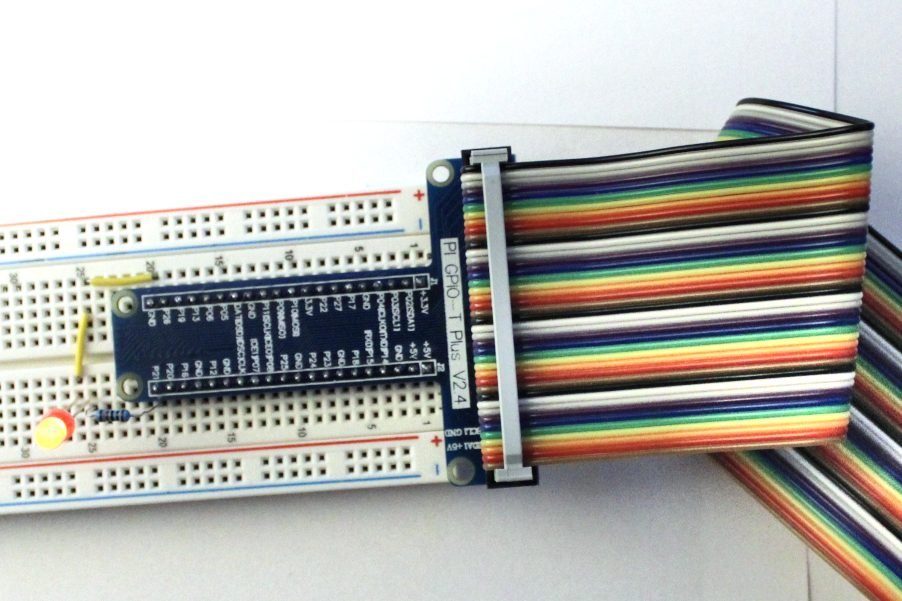
\includegraphics[width=\textwidth]{2-hardwaredesign/img/led_direkt_foto}
    \end{columns}
\end{frame}
}

%%% Folie
{
\footnotesize

\begin{frame}{Mittlere Lasten über Transistor schalten}
    \parbox{\linewidth}{
        Besser ist es daher, die Last über einen \textbf{Transistor} zu schalten. Der hier
        gezeigte \glqq{}npn-Transistor\grqq{} funktioniert wie ein \textbf{spannungsgesteuerter
        Schalter}. Liegt am mittleren Pin (der \glqq{}Basis\grqq{}) eine ausreichend hohe
        Spannung an, wird diese zusammen mit der am oberen Pin (dem \glqq{}Collector\grqq{})
        anliegenden Spannung auf den unteren Pin (dem \glqq{}Emitter\grqq{}) durchgelassen.
    }

    \bigskip

    \begin{columns}
        \column{0.5\textwidth}
        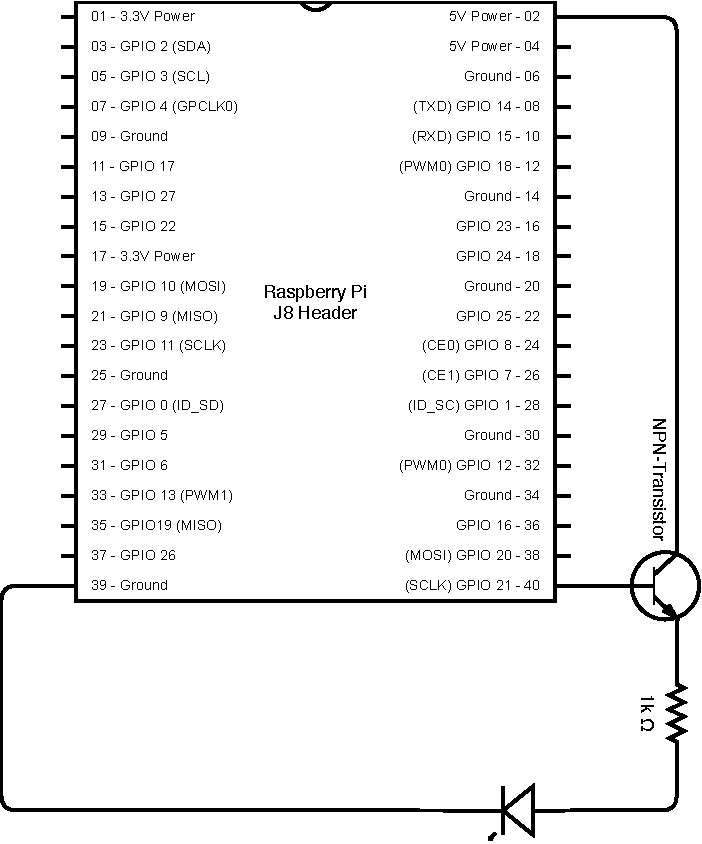
\includegraphics[width=.8\textwidth]{2-hardwaredesign/img/led_transistor_schaltplan}

        \column{0.5\textwidth}
        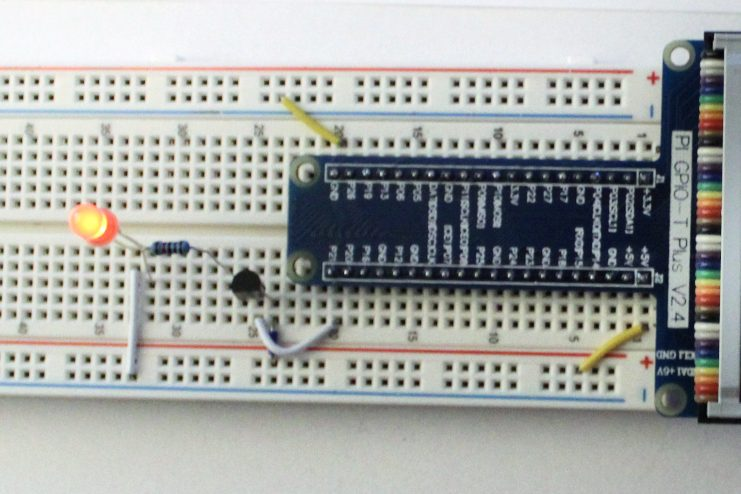
\includegraphics[width=\textwidth]{2-hardwaredesign/img/led_transistor_foto}
    \end{columns}
\end{frame}
}

%%% Folie
{
\footnotesize

\begin{frame}{Große Lasten über Relais schalten}
    \parbox{\linewidth}{
        Sehr große Lasten mit hoher Spannung und/oder hoher Stromstärke sollten aus
        Sicherheitsgründen galvanisch von der Mikrocontrollerschaltung entkoppelt werden, um
        bei einem Defekt nicht die gesamte Schaltung zu zerstören. Abhilfe schafft hier ein
        \textbf{Relais}, das als magnetischer Schalter den \textbf{Arbeitsstromkreis}
        schließt, sobald am \textbf{Steuerstromkreis} eine Spannung anliegt.
    }

    \bigskip

    \begin{columns}
        \column{0.5\textwidth}
        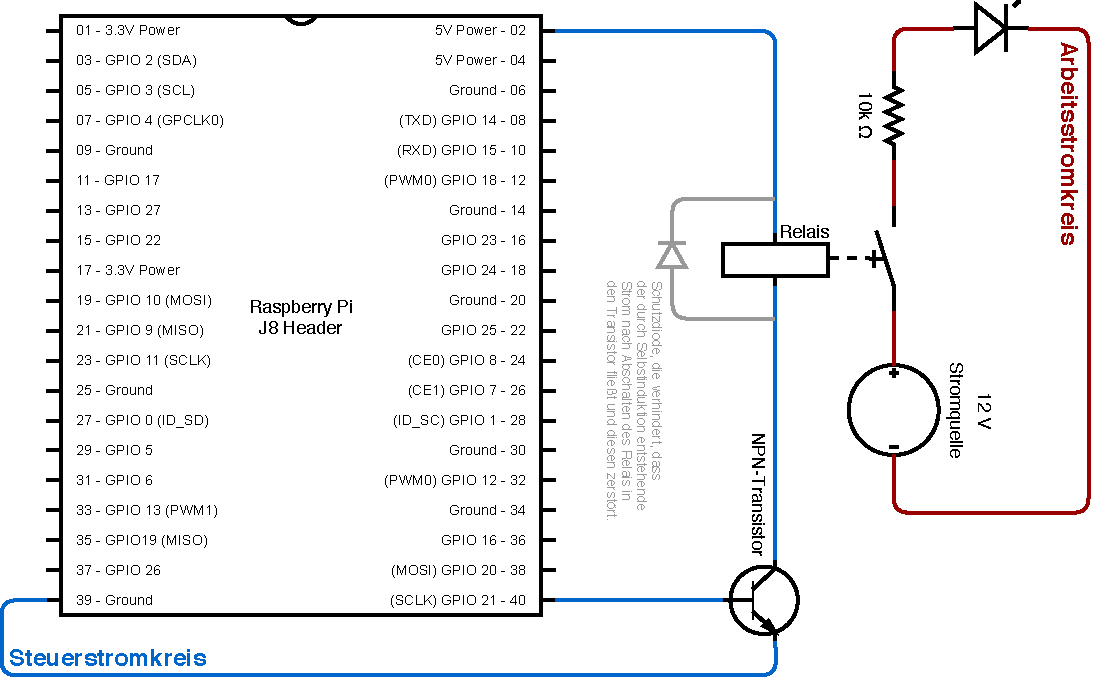
\includegraphics[width=\textwidth]{2-hardwaredesign/img/led_relais_schaltplan}

        \column{0.5\textwidth}
        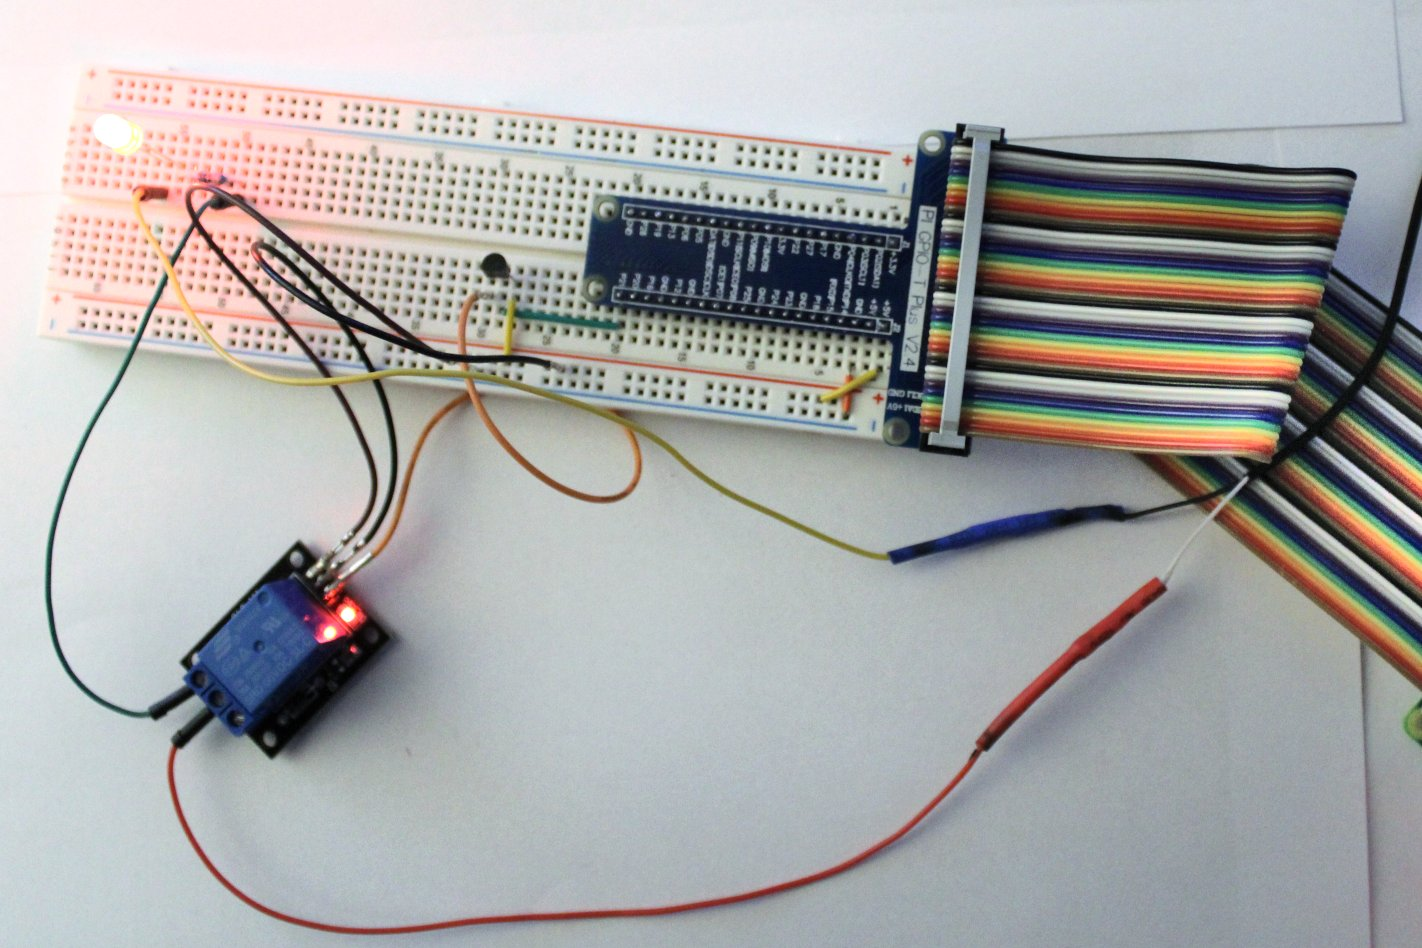
\includegraphics[width=\textwidth]{2-hardwaredesign/img/led_relais_foto}
    \end{columns}
\end{frame}
}

%%% Folie
{
\footnotesize

\begin{frame}{Gemittelte Leistung durch Pulsweitenmodulation regulieren}
    \parbox{\linewidth}{
        Die für eine Arbeit zur Verfügung stehende Stromstärke kann nicht nur durch Widerstände
        absolut reduziert werden. Sie kann durch \textbf{Pulsweitenmodulation} (schnelles Ein-
        und Ausschalten) auch im zeitlichen Mittel reduziert werden. Für kurze Zeit fließt dann
        zwar der volle Strom, die Länge der An- und Ausphasen reduziert jedoch die Gesamtstrommenge
        im zeitlichen Verlauf.
    }

    \begin{center}
        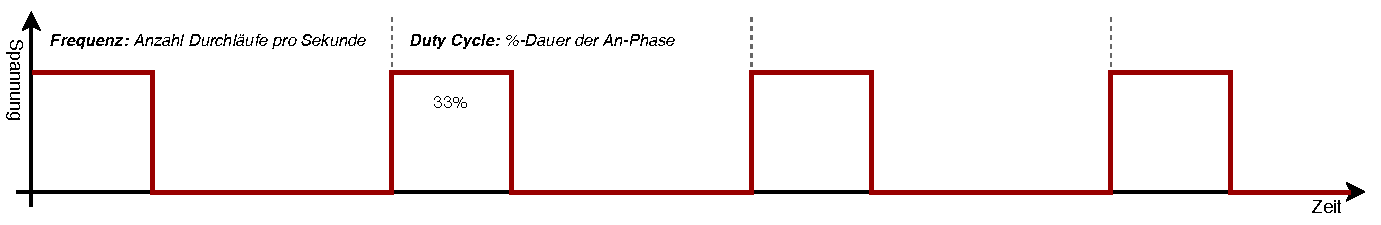
\includegraphics[width=.75\textwidth]{2-hardwaredesign/img/pwm}
    \end{center}

    \begin{columns}
        \column{.5\textwidth}
        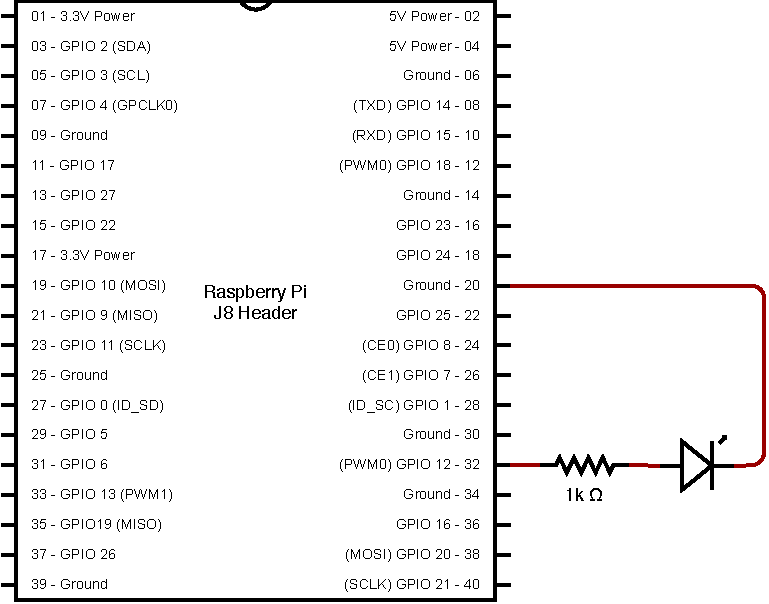
\includegraphics[width=.9\textwidth]{2-hardwaredesign/img/led_pwm_schaltplan}

        \column{.5\textwidth}
        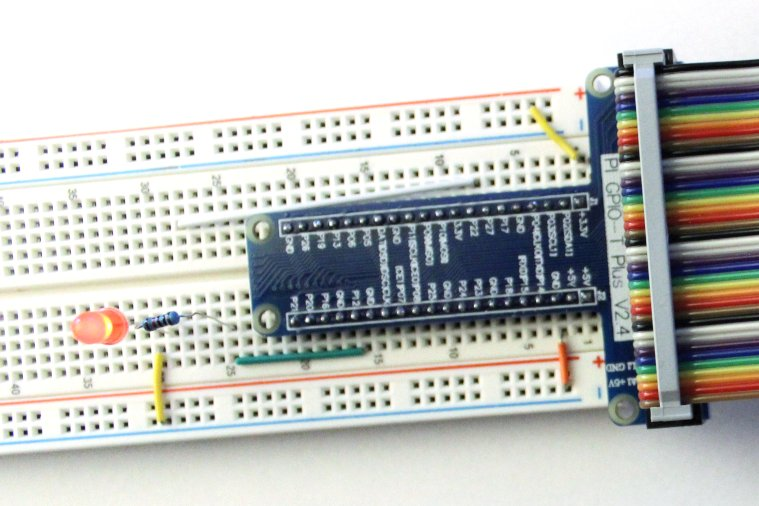
\includegraphics[width=\textwidth]{2-hardwaredesign/img/led_pwm_foto}
    \end{columns}
\end{frame}
}

%%% Folie
{
\footnotesize

\begin{frame}{Schließkontakt mit Pull-Down-Widerstand}
    \parbox{\linewidth}{
        Bisher haben wir nur gesehen, wie die GPIO-Pins als Ausgang und somit als schaltbare Stromquelle
        genutzt werden können. Jedoch können sie genauso gut auch als Eingang genutzt werden, um zu erkennen,
        wann ein Kontakt geschlossen wurde. Der hier gezeigte \textbf{Pull-Down-Widerstand} zieht das
        Eingangssignal dabei auf Masse (logisch Null) herunter, solange der Schalter nicht betätigt wird.
        Wird der Kontakt geschlossen, sieht der Raspberry Pi stattdessen eine logische Eins. In der Literatur
        findet sich hierfür auch die Bezeichnung \glqq{}Active High\grqq{}.
    }

    \bigskip

    \begin{columns}
        \column{0.5\textwidth}
        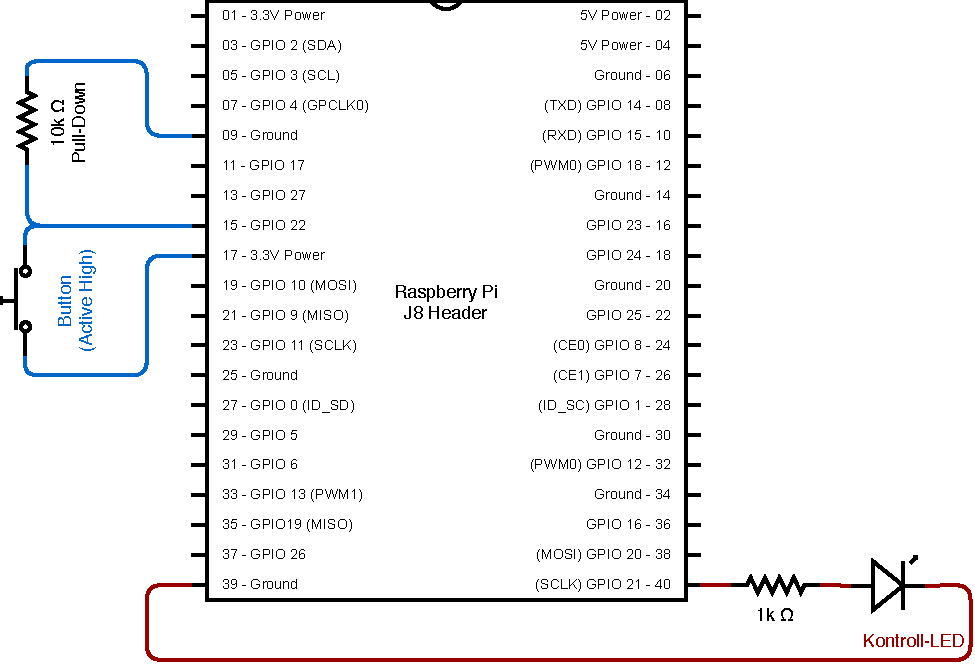
\includegraphics[width=\textwidth]{2-hardwaredesign/img/button_pulldown_schaltplan}

        \column{0.5\textwidth}
        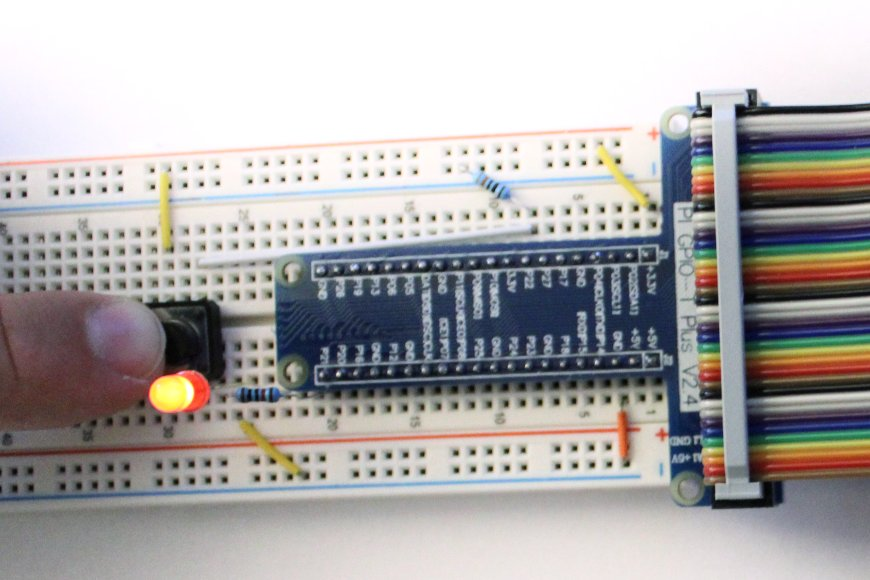
\includegraphics[width=\textwidth]{2-hardwaredesign/img/button_pulldown_foto}
    \end{columns}
\end{frame}
}

%%% Folie
{
\footnotesize

\begin{frame}{Schließkontakt mit Pull-Up-Widerstand}
    \parbox{\linewidth}{
        Das Gegenstück zum Pull-Down-Widerstand ist der \textbf{Pull-Up-Widerstand}. Hier
        zieht der Widerstand das Eingangssignal auf logisch Eins hoch, so dass der Raspberry
        so lange ein High-Signal sieht, bis der Schalter geschlossen wird. Dies wird in der
        Literatur oft auch \glqq{}Active Low\grqq{} genannt.
    }

    \bigskip

    \begin{columns}
        \column{0.5\textwidth}
        \includegraphics[width=\textwidth]{2-hardwaredesign/img/button_pullup_schaltplan}

        \column{0.5\textwidth}
        \includegraphics[width=\textwidth]{2-hardwaredesign/img/button_pullup_foto}
    \end{columns}
\end{frame}
}

%-------------------------------------------------------------------------------
\section{Integration komplexerer Bauteile}
%-------------------------------------------------------------------------------

%%% Folie
{
\tiny

\begin{frame}[allowframebreaks]{Beispiel: Sensorkit mit 40 Bauteilen}
    \begin{columns}
        \column{\dimexpr\paperwidth-28pt}
        \begin{center}
            \includegraphics[height=.8\textheight]{2-hardwaredesign/img/sensorkit_alle}
        \end{center}
    \end{columns}

    \begin{block}{Umweltsensoren}
        \medskip
        \begin{columns}
            \column{0.5\textwidth}
            KY-001: Temperatursensor (DS18B20) \\
            KY-002: Erschütterungsschalter \\
            KY-003: Hall Magnetfeldsensor \\
            KY-010: Lichtschranke \\
            KY-013: Temperatursensor \\
            KY-015: Temperatur, Feuchtigkeit (DHT11) \\
            KY-017: Neigungsschalter \\
            KY-018: Fotowiderstand \\
            KY-020: Neigungsschalter \\
            KY-021: Mini Magnet-Reedkontakt \\
            KY-024: Linear Magnetic Hall-Sensor \\
            KY-025: Reedkontakt \\
            KY-026: Flammensensor \\

            \column{0.5\textwidth}
            KY-027: Magic Light Cup  \\
            KY-028: Temperatursensor (Thermistor) \\
            KY-031: Klopfsensor \\
            KY-032: Hindernisdetektor \\
            KY-033: Trackingsensor \\
            KY-035: Bihor Magnetsensor \\
            KY-036: Metall-Touchsensor \\
            KY-037: Mikrofon Soundsensor \\
            KY-038: Mikrofon Soundsensor \\
            KY-039: Herzschlagsensor \\
            KY-050: Ultraschallabstandssensor \\
            KY-052: Drucksensor (BMP280) \\
        \end{columns}
    \end{block}

    \begin{block}{Ein-/Ausgabemodule}
        \medskip
        \begin{columns}
            \column{0.5\textwidth}
            KY-004: Taster \\
            KY-022: Infrarot-Receiver \\
            KY-023: XY-Joystick \\
            KY-040: Kodierter Drehschalter (Rotary Encoder) \\
            \smallskip
            KY-005: Infrarot-Transmitter \\
            KY-006: Passiver Piezo-Buzzer \\
            KY-009: RGB-LED (Surface-Mount) \\

            \column{0.5\textwidth}
            KY-011: 2-Farben (Rot und Grün) LED \\
            KY-012: Aktiver Piezo-Buzzer \\
            KY-016: RGB-LED (Through-Hole) \\
            KY-019: 5V Relais \\
            KY-029: 2-Farben (Rot und Grün) LED \\
            KY-034: 7-Farben LED \\
        \end{columns}
    \end{block}

    \begin{block}{Hilfsbausteine}
        \medskip
        \begin{columns}
            \column{0.5\textwidth}
            KY-051: Voltage Translator / Level Shifter \\

            \column{0.5\textwidth}
            KY-053: Analog/Digital Converter \\
        \end{columns}
    \end{block}
\end{frame}
}

{
\scriptsize

\begin{frame}{Module mit analoger Schnittstelle}
    \begin{columns}
        \column{.6\textwidth}
        \includegraphics[width=\textwidth]{2-hardwaredesign/img/sensorkit_analog}

        \column{.4\textwidth}
        KY-003: Hall Magnetfeldsensor \\
        KY-006: Passiver Piezo-Buzzer \\
        KY-009: RGB-LED (Surface-Mount) \\
        KY-011: 2-Farben (Rot und Grün) LED \\
        KY-012: Aktiver Piezo-Buzzer \\
        KY-013: Temperatursensor \\
        KY-016: RGB-LED (Through-Hole) \\
        KY-018: Fotowiderstand \\
        KY-023: XY-Joystick \\
        KY-024: Linear Magnetic Hall-Sensor \\
        KY-025: Reedkontakt \\
        KY-026: Flammensensor \\
        KY-028: Temperatursensor (Thermistor) \\
        KY-029: 2-Farben (Rot und Grün) LED \\
        KY-034: 7-Farben LED \\
        KY-035: Bihor Magnetsensor \\
        KY-036: Metall-Touchsensor \\
        KY-037: Mikrofon Soundsensor \\
        KY-038: Mikrofon Soundsensor \\
        KY-039: Herzschlagsensor \\
        KY-040: Kodierter Drehschalter \\
        KY-050: Ultraschallabstandssensor \\
    \end{columns}
\end{frame}

\begin{frame}{Module mit digitaler An/Aus-Schnittstelle}
    \begin{columns}
        \column{.6\textwidth}
        \includegraphics[width=\textwidth]{2-hardwaredesign/img/sensorkit_digital}

        \column{.4\textwidth}
        KY-002: Erschütterungsschalter \\
        KY-003: Hall Magnetfeldsensor \\
        KY-004: Taster \\
        KY-010: Lichtschranke \\
        KY-012: Aktiver Piezo-Buzzer \\
        KY-017: Neigungsschalter \\
        KY-019: 5V Relais \\
        KY-020: Neigungsschalter \\
        KY-021: Mini Magnet-Reedkontakt \\
        KY-024: Linear Magnetic Hall-Sensor \\
        KY-025: Reedkontakt \\
        KY-026: Flammensensor \\
        KY-027: Magic Light Cup \\
        KY-028: Temperatursensor (Thermistor) \\
        KY-031: Klopfsensor \\
        KY-032: Hindernisdetektor \\
        KY-033: Trackingsensor \\
        KY-036: Metall-Touchsensor \\
        KY-037: Mikrofon Soundsensor \\
        KY-038: Mikrofon Soundsensor \\
    \end{columns}
\end{frame}

\begin{frame}{Module mit serieller Schnittstelle}
    \begin{columns}
        \column{.6\textwidth}
        \includegraphics[width=\textwidth]{2-hardwaredesign/img/sensorkit_seriell}

        \column{.4\textwidth}
        KY-001: Temperatursensor (DS18B20) \\
        KY-015: Temperatur, Feuchtigkeit (DHT11) \\
        KY-052: Drucksensor (BMP280) \\
        KY-053: Analog/Digital Converter \\
    \end{columns}
\end{frame}
}

%%% Folie
{
\scriptsize

\begin{frame}{Beispiel: DHT11-Sensor über 1-wire}
    Der DHT11-Sensor misst alle zwei Sekunden Temperatur und relative Luftfeuchtigkeit. \\
    Die Werte werden über das serielle 1-wire-Protokoll als digitaler Datenstrom übertragen. \\
    \medskip

    \begin{center}
        \includegraphics[width=.8\textwidth]{2-hardwaredesign/img/dht11_schaltplan}
    \end{center}
\end{frame}
}

{
    \setbeamertemplate{background canvas}{
        \includegraphics[height=\paperheight, width=\paperwidth]{2-hardwaredesign/img/dht11_foto1}
    }

    \begin{frame}[plain]
    \end{frame}
}

{
    \setbeamertemplate{background canvas}{
        \includegraphics[height=\paperheight, width=\paperwidth]{2-hardwaredesign/img/dht11_foto2}
    }

    \begin{frame}[plain]
    \end{frame}
}

%%% Folie
{
\small

\begin{frame}{Weitere serielle Schnittstellen}
    \begin{columns}
        \column[T]{.5\textwidth}
        \textbf{Universal Asynchronous Receiver Transmitter (UART)} \\
        \smallskip
        \includegraphics[width=\textwidth]{2-hardwaredesign/img/seriell_uart_schaltplan}

        \column[T]{.5\textwidth}
        \textbf{Serial Peripheriel Interface (SPI)} \\
        \smallskip
        \includegraphics[width=0.8\textwidth]{2-hardwaredesign/img/seriell_spi_schaltplan}
    \end{columns}

    \medskip

    \textbf{Inter-Integrated Circuit (I²C)} \\
    \smallskip
    \includegraphics[width=\textwidth]{2-hardwaredesign/img/seriell_i2c_schaltplan}
\end{frame}
}

%%% Folie
\begin{frame}{Einsatzgebiete serieller Schnittstellen}
    \begin{columns}
        \column{\dimexpr\paperwidth-28pt}
        \begin{itemize}
            \item Kommunikation zwischen den Komponenten eines eingebetteten Systems
            \item Datenaustausch zwischen getrennten Subsystemen und anderen Computern
            \item Anbindung von Sensoren und Aktoren an Eingebettete/IoT-Devices
        \end{itemize}
    \end{columns}

    \bigskip
    \bigskip
    \bigskip

    \begin{columns}
        \column{.33\textwidth}
        \includegraphics[width=\textwidth]{2-hardwaredesign/img/seriell_einsatz1}

        \column{.33\textwidth}
        \includegraphics[width=\textwidth]{2-hardwaredesign/img/seriell_einsatz2}

        \column{.33\textwidth}
        \includegraphics[width=\textwidth]{2-hardwaredesign/img/seriell_einsatz3}
    \end{columns}
\end{frame}
